% Judul dokumen
\title{Buku Tugas Akhir ITS}
\author{Amiri, Aufa}

% Pengaturan ukuran teks dan bentuk halaman dua sisi
\documentclass[10pt,twoside]{report}

% Pengaturan ukuran halaman dan margin
\usepackage[a5paper,top=25mm,left=25mm,right=20mm,bottom=25mm]{geometry}

% Pengaturan ukuran spasi
\usepackage[singlespacing]{setspace}

% Pengaturan format bahasa
\usepackage[indonesian]{babel}

\usepackage[hyphens]{url}
% Pengaturan detail pada file PDF
\usepackage[pdfauthor={\@author},bookmarksnumbered,pdfborder={0 0 0}, breaklinks]{hyperref}


% Pengaturan jenis karakter
\usepackage[utf8]{inputenc}

% Pengaturan pewarnaan
\usepackage[table,xcdraw]{xcolor}

% Pengaturan kutipan artikel
\usepackage[numbers]{natbib}

% Package lainnya
\usepackage{changepage}
\usepackage{enumitem}
\usepackage{eso-pic}
\usepackage{etoolbox}
\usepackage{graphicx}
\usepackage{lipsum}
\usepackage{lmodern}
\usepackage{longtable}
\usepackage{tabularx}
\usepackage{wrapfig}
\usepackage{amsmath}

% Definisi untuk "Hati ini sengaja dikosongkan"
\patchcmd{\cleardoublepage}{\hbox{}}{
  \thispagestyle{empty}
  \vspace*{\fill}
  \begin{center}\textit{[Halaman ini sengaja dikosongkan]}\end{center}
  \vfill}{}{}

% Pengaturan penomoran halaman
\usepackage{fancyhdr}
\fancyhf{}
\renewcommand{\headrulewidth}{0pt}
\pagestyle{fancy}
\fancyfoot[CE,CO]{\thepage}
\patchcmd{\chapter}{plain}{fancy}{}{}
\patchcmd{\chapter}{empty}{plain}{}{}

% Pengaturan format judul bab
\usepackage{titlesec}
\titleformat{\chapter}[display]{\bfseries\Large}{BAB \centering\arabic{chapter}}{0ex}{\vspace{0ex}\centering}
\titleformat{\section}{\bfseries\large}{\MakeUppercase{\thesection}}{1ex}{\vspace{1ex}}
\titleformat{\subsection}{\bfseries\large}{\MakeUppercase{\thesubsection}}{1ex}{}
\titleformat{\subsubsection}{\bfseries\large}{\MakeUppercase{\thesubsubsection}}{1ex}{}
\titlespacing{\chapter}{0ex}{0ex}{4ex}
\titlespacing{\section}{0ex}{1ex}{0ex}
\titlespacing{\subsection}{0ex}{0.5ex}{0ex}
\titlespacing{\subsubsection}{0ex}{0.5ex}{0ex}

% Pengaturan format potongan kode
\usepackage{listings}
\definecolor{comment}{RGB}{0,128,0}
\definecolor{string}{RGB}{255,0,0}
\definecolor{keyword}{RGB}{0,0,255}
\lstdefinestyle{codestyle}{
  commentstyle=\color{comment},
  stringstyle=\color{string},
  keywordstyle=\color{keyword},
  basicstyle=\footnotesize\ttfamily,
  numbers=left,
  numberstyle=\tiny,
  numbersep=5pt,
  frame=lines,
  breaklines=true,
  prebreak=\raisebox{0ex}[0ex][0ex]{\ensuremath{\hookleftarrow}},
  showstringspaces=false,
  upquote=true,
  tabsize=2,
}
\lstset{style=codestyle}

\hyphenation{ Re-pre-sen-ta-tions }

% Isi keseluruhan dokumen
\begin{document}

% Sampul luar Bahasa Indonesia
\newcommand\covercontents{sampul/konten-id.tex}
\AddToShipoutPictureBG*{
  \AtPageLowerLeft{
    % Ubah nilai berikut jika posisi horizontal background tidak sesuai
    \hspace{-3.5mm}

    % Ubah nilai berikut jika posisi vertikal background tidak sesuai
    \raisebox{0mm}{
      
\includegraphics[width=\paperwidth,height=\paperheight]{sampul/gambar/sampul-luar.png}
    }
  }
}

% Menyembunyikan nomor halaman
\thispagestyle{empty}

% Pengaturan margin untuk menyesuaikan konten sampul
\newgeometry{
  top=95mm,
  left=25mm,
  right=20mm,
  bottom=25mm
}

\begin{flushleft}

  % Pemilihan font sans serif
  \sffamily

  % Pemilihan warna font putih
  \color{white}

  % Pemilihan font bold
  \fontseries{bx}
  \selectfont

  \input{\covercontents}

\end{flushleft}

\restoregeometry


%Setup Table
\renewcommand{\arraystretch}{1.5}

% Atur ulang penomoran halaman
\setcounter{page}{1}

% Sampul dalam Bahasa Indonesia
\renewcommand\covercontents{sampul/konten-id.tex}
\AddToShipoutPictureBG*{
  \AtPageLowerLeft{
    % Ubah nilai berikut jika posisi horizontal background tidak sesuai
    \hspace{-3.5mm}

    % Ubah nilai berikut jika posisi vertikal background tidak sesuai
    \raisebox{0mm}{
      
\includegraphics[width=\paperwidth,height=\paperheight]{sampul/gambar/sampul-dalam.png}
    }
  }
}

% Menyembunyikan nomor halaman
\thispagestyle{empty}

% Pengaturan margin untuk menyesuaikan konten sampul
\newgeometry{
  top=95mm,
  left=25mm,
  right=20mm,
  bottom=25mm
}

\begin{flushleft}

  % Pemilihan font sans serif
  \sffamily

  % Pemilihan font bold
  \fontseries{bx}
  \selectfont

  \input{\covercontents}

\end{flushleft}

\restoregeometry

\clearpage
\cleardoublepage

% Sampul dalam Bahasa Inggris
\renewcommand\covercontents{sampul/konten-en.tex}
\AddToShipoutPictureBG*{
  \AtPageLowerLeft{
    % Ubah nilai berikut jika posisi horizontal background tidak sesuai
    \hspace{-3.5mm}

    % Ubah nilai berikut jika posisi vertikal background tidak sesuai
    \raisebox{0mm}{
      
\includegraphics[width=\paperwidth,height=\paperheight]{sampul/gambar/sampul-dalam.png}
    }
  }
}

% Menyembunyikan nomor halaman
\thispagestyle{empty}

% Pengaturan margin untuk menyesuaikan konten sampul
\newgeometry{
  top=95mm,
  left=25mm,
  right=20mm,
  bottom=25mm
}

\begin{flushleft}

  % Pemilihan font sans serif
  \sffamily

  % Pemilihan font bold
  \fontseries{bx}
  \selectfont

  \input{\covercontents}

\end{flushleft}

\restoregeometry

\cleardoublepage

% Pengaturan ukuran indentasi paragraf
\setlength{\parindent}{2em}

% Pengaturan ukuran spasi paragraf
\setlength{\parskip}{1ex}

% Pernyataan keaslian
% \begin{center}
  \large
  \textbf{PERNYATAAN KEASLIAN\\TUGAS AKHIR}
\end{center}

% Menyembunyikan nomor halaman
\thispagestyle{empty}

\vspace{2ex}

% Ubah paragraf-paragraf berikut sesuai dengan yang ingin diisi pada pernyataan keaslian

Dengan ini saya menyatakan bahwa isi buku Tugas Akhir \lipsum[1][1-6]

Semua referensi yang dikutip maupun dirujuk telah \lipsum[2][1-4]

\vspace{4ex}

\begin{flushright}
  \begin{tabular}[b]{c}
    % Ubah kalimat berikut sesuai dengan tempat, bulan, dan tahun penulisan
    Surabaya, Mei 2021\\
    \\
    \\
    \\
    \\
    % Ubah kalimat-kalimat berikut sesuai dengan nama dan NRP mahasiswa
    Elon Reeve Musk\\
    0123 20 4000 0001
  \end{tabular}
\end{flushright}

% \cleardoublepage

% Lembar pengesahan
% \begin{center}
  \large
  \textbf{LEMBAR PENGESAHAN}
\end{center}

% Menyembunyikan nomor halaman
\thispagestyle{empty}

\begin{center}
  % Ubah kalimat berikut dengan judul tugas akhir
  \textbf{DETEKSI BERITA PALSU OTOMATIS BERBAHASA INDONESIA MENGGUNAKAN BERT}
\end{center}

\begingroup
% Pemilihan font ukuran small
\small

\begin{center}
  % Ubah kalimat berikut dengan pernyataan untuk lembar pengesahan
  Tugas Akhir ini disusun untuk memenuhi salah satu syarat memperoleh gelar Sarjana Teknik di Institut Teknologi Sepuluh Nopember Surabaya

\end{center}

\begin{center}
  % Ubah kalimat berikut dengan nama dan NRP mahasiswa
  Oleh: Aufa Nabil Amiri (NRP. 0721 17 4000 0029)
\end{center}

\begingroup
% Menghilangkan padding
\setlength{\tabcolsep}{0pt}

\noindent
\begin{tabularx}{\textwidth}{X c}
  Tanggal Ujian : Juli 2020                                                    & Periode Wisuda : September 2020 \\
                                                                               &                                 \\
  Disetujui oleh :                                                             &                                 \\
  % Ubah kalimat-kalimat berikut dengan nama dan NIP dosen pembimbing pertama
  \underline{Reza Fuad Rachmadi ST., MT., Ph. D} \newline
  NIP: 19850403 201212 1 001                                                   & (Pembimbing I)                  \\ \\
  % Ubah kalimat-kalimat berikut dengan nama dan NIP dosen pembimbing kedua
  \underline{Prof. Dr. Ir. Mauridhy Hery Purno-} \newline \underline{mo, M. Eng} \newline NIP: 19580916 198601 1 001
                                                                               & (Pembimbing II)                 \\ \\
  % Ubah kalimat-kalimat berikut dengan nama dan NIP dosen penguji pertama
  \underline{Dr. Surya Supemo, S.T., M.T.} \newline NIP. 19690613 199702 1 003 & (Penguji I)                     \\ \\

  % Ubah kalimat-kalimat berikut dengan nama dan NIP dosen penguji kedua
  \underline{Eko Pramunanto, S.T., M.T.} \newline NIP. 19661203 199412 1 001   & (Penguji II)                    \\ \\

  % Ubah kalimat-kalimat berikut dengan nama dan NIP dosen penguji ketiga
  \underline{Dion Hayu Fandiantoro} \newline NIP. 19942020 11064               & (Penguji III)                   \\
\end{tabularx}
\endgroup

\begin{center}
  % Ubah kalimat berikut dengan jabatan kepala departemen
  Mengetahui, \\
  Kepala Departemen Teknik Komputer FTEIC - ITS \\

  \vspace{7ex}

  % Ubah kalimat-kalimat berikut dengan nama dan NIP kepala departemen
  \underline{Dr. Supeno Mardi Susiki Nugroho, ST., MT.} \\
  NIP. 19700313 199512 1 001
\end{center}
\endgroup

% \cleardoublepage

% Nomor halaman pembuka dimulai dari sini
\pagenumbering{roman}

% Abstrak Bahasa Indonesia
\begin{center}
  \large\textbf{ABSTRAK}
\end{center}

\addcontentsline{toc}{chapter}{ABSTRAK}

\vspace{2ex}

\begingroup
% Menghilangkan padding
\setlength{\tabcolsep}{0pt}

\noindent
\begin{tabularx}{\textwidth}{l >{\centering}m{2em} X}
  % Ubah kalimat berikut dengan nama mahasiswa
  Nama Mahasiswa    & : & Aufa Nabil Amiri                                                   \\

  % Ubah kalimat berikut dengan judul tugas akhir
  Judul Tugas Akhir & : & Deteksi Berita Palsu Otomatis Berbahasa Indonesia Menggunakan BERT \\

  % Ubah kalimat-kalimat berikut dengan nama-nama dosen pembimbing
  Pembimbing        & : & 1. Reza Fuad Rachmadi ST., MT., Ph.D                               \\
                    &   & 2. Prof. Dr. Ir. Mauridhi Hery Purnomo, M. Eng                     \\
\end{tabularx}
\endgroup

% Ubah paragraf berikut dengan abstrak dari tugas akhir
Berita palsu atau yang biasa disebut hoaks adalah suatu yang hal yang sering melanda Indonesia. Dengan adanya sosial media, suatu berita palsu dapat memiliki tingkat penyebaran yang sangat luas. Selain itu, masyarakat Indonesia memiliki tingkat kecenderungan untuk menyebarkan berita palsu yang cukup tinggi. Sehingga, suatu metode pendeteksi berita palsu harus ada. Penelitian ini memanfaatkan algoritma BERT yang digunakan untuk mendeteksi apakah suatu berita adalah berita hoaks atau tidak secara otomatis. Dari suatu teks yang mentah, akan dilakukan tokenisasi sebelum akhirnya dimasukkan ke dalam algoritma BERT. Selanjutnya, keluaran dari BERT akan dijadikan sebagai inputan dari algoritma klasifikasi Linear Regression.  Barulah pada saat ini, kita bisa mendapatkan klasifikasi apakah suatu teks itu berupa berita hoaks atau tidak. Tujuan dari penelitian ini adalah untuk membuat sebuah model yang dapat digunakan untuk melakukan klasifikasi suatu teks apakah termasuk ke dalam berita hoaks atau tidak. Hasil dari penelitian ini adalah model yang dapat mendeteksi berita hoaks dengan tingkat akurasi sebesar 89\%.

% Ubah kata-kata berikut dengan kata kunci dari tugas akhir
Kata Kunci:   BERT, Hoaks, Klasifikasi, Linear Regression.

\cleardoublepage

% Abstrak Bahasa Inggris
\begin{center}
  \large\textbf{ABSTRACT}
\end{center}

\addcontentsline{toc}{chapter}{ABSTRACT}

\vspace{2ex}

\begingroup
% Menghilangkan padding
\setlength{\tabcolsep}{0pt}

\noindent
\begin{tabularx}{\textwidth}{l >{\centering}m{3em} X}
  % Ubah kalimat berikut dengan nama mahasiswa
  \emph{Name}     & : & Aufa Nabil Amiri                                             \\

  % Ubah kalimat berikut dengan judul tugas akhir dalam Bahasa Inggris
  \emph{Title}    & : & \emph{ Automatic Indonesian Hoax News Detection Using BERT } \\

  % Ubah kalimat-kalimat berikut dengan nama-nama dosen pembimbing
  \emph{Advisors} & : & 1. Reza Fuad Rachmadi, S.T., M.T., Ph.D                      \\
                  &   & 2. Prof. Dr. Ir. Mauridhi Hery Purnomo, M. Eng               \\
\end{tabularx}
\endgroup

% Ubah paragraf berikut dengan abstrak dari tugas akhir dalam Bahasa Inggris
\textit{
  Fake news or usually called hoax, is one of things that ofen plaguing Indonesia. With a social media, a fake news can spread wider and faster than ever before. On another note, Indonesian people have quite a high tendencies to share fake news. Based on that note, we are in dire need of a method to detect fake news. This research is using BERT method to automatically detect whether a news can be considered as hoax or not. From a raw text, we are doing a tokenization process before we feed the text to the BERT method. Next, the pooled output of the BERT is being used as the input for Linear Regression, a tested-and-true method for classifying task. Now that we have pass-through all  those steps, we can determine whether a text is a hoax or not. The purpose of this research is to create a machine learning model to help the people to determine whether a text can be considered as hoax or not.
}

% Ubah kata-kata berikut dengan kata kunci dari tugas akhir dalam Bahasa Inggris
\emph{Keywords}: \emph{BERT}, \emph{Hoax}, \emph{Fake News} \emph{Classification}, \emph{Linear Regression}.

\cleardoublepage

% Kata pengantar
% \begin{center}
  \Large
  \textbf{KATA PENGANTAR}
\end{center}

\addcontentsline{toc}{chapter}{KATA PENGANTAR}

\vspace{2ex}

% Ubah paragraf-paragraf berikut dengan isi dari kata pengantar

Puji dan syukur kehadirat \lipsum[1][1-5]

Penelitian ini disusun dalam rangka \lipsum[2][1-5]
Oleh karena itu, penulis mengucapkan terima kasih kepada:

\begin{enumerate}[nolistsep]

  \item Keluarga, Ibu, Bapak dan Saudara tercinta yang telah \lipsum[3][1-2]

  \item Bapak Nikola Tesla, S.T., M.T., selaku \lipsum[4][1-2]

  \item \lipsum[5][1-3]

\end{enumerate}

Akhir kata, semoga \lipsum[6][1-8]

\begin{flushright}
  \begin{tabular}[b]{c}
    % Ubah kalimat berikut dengan tempat, bulan, dan tahun penulisan
    Surabaya, Mei 2021\\
    \\
    \\
    \\
    \\
    % Ubah kalimat berikut dengan nama mahasiswa
    Elon Reeve Musk
  \end{tabular}
\end{flushright}

% \cleardoublepage

% Daftar isi
\renewcommand*\contentsname{DAFTAR ISI}
\addcontentsline{toc}{chapter}{\contentsname}
\tableofcontents
\cleardoublepage

% Daftar gambar
\renewcommand*\listfigurename{DAFTAR GAMBAR}
\addcontentsline{toc}{chapter}{\listfigurename}
\listoffigures
\cleardoublepage

% Daftar tabel
\renewcommand*\listtablename{DAFTAR TABEL}
\addcontentsline{toc}{chapter}{\listtablename}
\listoftables
\cleardoublepage

% Nomor halaman isi dimulai dari sini
\pagenumbering{arabic}

% Bab 1 pendahuluan
\chapter{PENDAHULUAN}
\label{chap:pendahuluan}

% Ubah bagian-bagian berikut dengan isi dari pendahuluan

Penelitian ini dilatar belakangi oleh berbagai kondisi yang menjadi acuan. Selain itu juga terdapat beberapa permasalahan yang akan dijawab sebagai luaran dari penelitian.

\section{Latar Belakang}
\label{sec:latarbelakang}

Pesatnya perkembangan roket yang merupakan \lipsum[1]

\lipsum[2]

\section{Permasalahan}
\label{sec:permasalahan}

Dari permasalahan tersebut maka \lipsum[1][1-6]

\section{Tujuan}
\label{sec:Tujuan}

Tujuan dari \lipsum[1][1-3] adalah:

\begin{enumerate}[nolistsep]

  \item Membuat \lipsum[2][1-3]

  \item \lipsum[3][1-3]

\end{enumerate}

\section{Batasan Masalah}
\label{sec:batasanmasalah}

Batasan-batasan dari \lipsum[1][1-3] adalah:

\begin{enumerate}[nolistsep]

  \item Mempermudah \lipsum[2][1-3]

  \item \lipsum[3][1-5]

  \item \lipsum[4][1-5]

\end{enumerate}

\section{Sistematika Penulisan}
\label{sec:sistematikapenulisan}

Laporan penelitian tugas akhir ini terbagi menjadi \lipsum[1][1-3] yaitu:

\begin{enumerate}[nolistsep]

  \item \textbf{BAB I Pendahuluan}

  Bab ini berisi \lipsum[2][1-5]

  \vspace{2ex}

  \item \textbf{BAB II Tinjauan Pustaka}

  Bab ini berisi \lipsum[3][1-5]

  \vspace{2ex}

  \item \textbf{BAB III Desain dan Implementasi Sistem}

  Bab ini berisi \lipsum[4][1-5]

  \vspace{2ex}

  \item \textbf{BAB IV Pengujian dan Analisa}

  Bab ini berisi \lipsum[5][1-5]

  \vspace{2ex}

  \item \textbf{BAB V Penutup}

  Bab ini berisi \lipsum[6][1-5]

\end{enumerate}

\cleardoublepage

% Bab 2 tinjauan pustaka
\chapter{TINJAUAN PUSTAKA}
\label{chap:tinjauanpustaka}

% Ubah bagian-bagian berikut dengan isi dari tinjauan pustaka
Demi mendukung penelitian ini, dibutuhkan beberapa teori penunjang sebagai bahan acuan dan referensi. Dengan demikian penelitian ini menjadi lebih terarah.

\section{Berita Palsu}
\label{sec:beritapalsu}

Berita palsu atau biasa dikenal dengan berita hoaks adalah sebuah informasi yang sesungguhnya tidak benar, tetapi dibuat seolah - olah benar adanya \cite{berita_bohong}. Di Indonesia sendiri, hoaks menjadi sebuah masalah tersendiri, hal ini karena masih banyak masyarakat yang langsung mempercayai apapun yang mereka temui di internet tanpa melakukan cek fakta terlebih dahulu.

Ada banyak sekali efek dari berita palsu ini, mulai dari hilangnya reputasi sampai nyawa yang terancam. Salah satu contoh kasus yang cukup parah adalah kerusuhan yang terjadi di Papua, dimana kerusuhan tersebut disebabkan karena adanya hoaks soal ucapan rasialis dari seorang guru SMP kepada muridnya \cite{efek_hoax}.

\section{\textit{Machine Learning}}

\textit{Machine Learning} atau Pembelajaran Mesin adalah salah satu cabang dalam kecerdasan buatan dan ilmu komputer yang menggunakan data dan algoritma untuk meniru manusia dalam mempelajari sesuatu \cite{ibm_ml_expl}. Salah satu hal yang membuat pembelajaran mesin sangat diminati adalah kemampuannya untuk menyelesaikan suatu tugas dengan sedikit intervensi dari manusia.

Sekarang ini, pembelajaran mesin adalah salah satu fokus yang cukup diminati pada bidang \textit{data science}. Dimana dengan menggunakan pembelajaran mesin, diharapkan suatu kecerdasan buatan dapat menyelesaikan beberapa tugas yang bagi komputer cukup rumit seperti misalnya, memberikan prediksi yang akurat berdasarkan data, melakukan klasifikasi pada teks maupun pada gambar, melakukan pemrosesan citra guna mengenali objek di dalam citra tersebut, dan masih banyak lagi.

Untuk prosesnya sendiri, awalnya kita harus mengumpulkan data, data ini dapat kita ambil dari  berbagai sumber atau bisa juga menggunakan data yang berasal dari instansi atau pribadi (data yang kita buat sendiri). Selanjutnya adalah proses \textit{training} dimana data akan dimasukkan ke dalam model pembelajaran mesin yang sudah dipilih. Kita dapat merubah beberapa parameter dari model tersebut untuk meningkatkan akurasi dari suatu model pembelajaran mesin. Terakhir adalah melakukan proses \textit{testing}, dimana model akan melakukan prediksi pada set data yang berbeda dari yang digunakan pada saat proses \textit{training}. Apabila ternyata tingkat akurasi dirasa kurang memadai, dapat dilakukan proses \textit{re-training} sampai tingkat akurasi nya dirasa cukup. Hasil akhir dari proses ini adalah sebuah model pembelajaran mesin yang dapat digunakan walaupun menggunakan data yang berbeda \cite{mit_ml_expl}.

\subsection{\textit{Supervised Learning}}

Salah satu cabang dalam bidang pembelajaran mesin. Disini data yang dijadikan masukan ke model sudah diberikan label atau struktur tertentu \cite{ms_ml_expl}. Berdasarkan dari data berlabel tersebut, sebuah model akan merubah parameter internalnya agar mendekati atau sesuai dengan label yang diberikan \cite{ibm_ml_expl}. Salah satu contoh model pembelajaran mesin dengan metode pembelajaran seperti ini adalah \textit{Linear Regression, Random Forest}, dan sebagainya.

\subsection{\textit{Unsupervised Learning}}

Salah satu cabang dalam bidang pembelajaran mesin. Disini data yang dijadikan masukan ke model tidak diberikan label sama sekali. Nantinya model akan membuat pengelompokan (\textit{clusters}) dan hubungan berdasarkan dari data yang diberikan \cite{mit_ml_expl}. Contoh model yang menggunakan metode pembelajaran ini adalah \textit{BERT, GPT-2/3} dan sebagainya.

\subsection{\textit{Reinforcement Learning}}

Salah satu cabang dalam bidang pembelajaran mesin. Disini model tidak diberikan data awal sama sekali, namun, model dibiarkan melakukan proses percobaan secara mandiri terus-menerus sampai tercapai hasil atau respon yang diinginkan. Apabila terdapat parameter yang menghasilkan respon positif, maka parameter tersebut disimpan dan digunakan sebagai masukan untuk iterasi \textit{training} berikutnya \cite{mit_ml_expl}.

\section{\textit{Deep Learning}}

Mirip seperti pembelajaran mesin, \textit{Deep Learning} juga merupakan salah satu bidang dalam bidang kecerdasan buatan. Yang membedakan antara pembelajaran mesin biasa dengan \textit{deep learning} adalah penggunaan \textit{layer} yang sangat banyak dibandingkan dengan pembelajaran mesin yang hanya memiliki 3 \textit{layers}. Keuntungan dari model jenis ini adalah model ini dapat memproses masukan yang paling abstrak sekalipun, sehingga menghilangkan proses ekstraksi fitur secara manual \cite{mathwork_deeplearning}. Namun, karena \textit{deep learning} memiliki \textit{layers} yang sangat banyak, maka diperlukan jumlah data yang jauh lebih banyak pula, karena itu pulalah, sebuah model \textit{deep learning} memerlukan daya komputasi yang jauh lebih besar dibandingkan dengan model pembelajaran mesin biasa \cite{mit_ml_expl}.

Gambar \ref{fig: deeplearning_layer} merupakan contoh bentuk \textit{layer} dalam suatu model \textit{deep learning} yang menggunakan 4 \textit{layers} didalamnya. Setiap \textit{layer} dapat memiliki fungsi dan tanggung jawabnya masing - masing \cite{mit_ml_expl}, seperti misal apabila kita menggunakan \textit{deep learning} untuk mendeteksi angka plat nomor di kendaraan bermotor, bisa saja beberapa layer pertama berfungsi untuk mendeteksi letak plat nomor dalam suatu citra, kemudian beberapa layer selanjutnya berfungsi untuk mengambil bentuk dari setiap objek dalam plat nomor tersebut, beberapa layer terakhir berfungsi untuk mengenali bentuk - bentuk dari objek menjadi tulisan teks. Semakin banyak layer yang digunakan, maka semakin tinggi pula kemungkinan kita melakukan sesuatu yang lebih kompleks \cite{mit_ml_expl}.

\begin{figure}[ht]
    \centering
    % Ubah file gambar berikut dengan file foto dari mahasiswa
    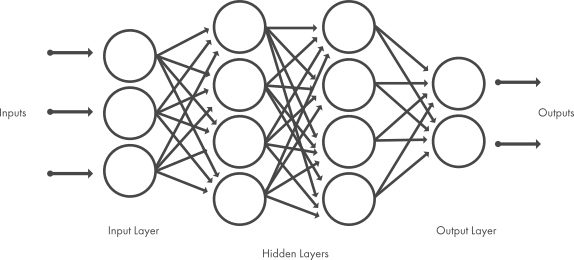
\includegraphics[width=\textwidth]{gambar/deeplearning_layer.png}
    \caption{Contoh \textit{Deep Learning} dengan 4 layer \cite{mathwork_deeplearning}}
    \label{fig: deeplearning_layer}
\end{figure}

\section{\textit{Transformer}}

\textit{Transformer} merupakan model \textit{deep learning} yang dibuat pada oleh Vaswani et. al, pada penelitian yang berjudul "Attention Is All You Need". \textit{Transformer} sendiri adalah sebuah arsitektur model yang berguna untuk merubah teks menjadi suatu bentuk yang lain bergantung pada tujuan implementasi model tersebut \cite{attention_is_all_you_need}. Tujuan dari \textit{transformer} sendiri sebagai pengembangan dari model rekuren (\textit {Recurrent Neural Network(RNN), Long Short-Term Memory(LSTM)}) ditambah dengan metode \textit{attention span} yang biasanya digunakan untuk melakukan suatu tugas dimana model harus "mengingat" masukan sebelumnya. Model rekuren seperti ini sangat berguna untuk suatu masukan yang bersifat sekuensial, seperti teks atau video sehingga sangat cocok untuk tugas yang memproses banyak teks seperti \textit{Natural Language Understanding (NLU)} atau mesin translasi otomatis \cite{lion_transformer}.

Namun, kelemahan yang cukup fatal adalah ketidakmampuan model rekuren ini untuk memproses data secara paralel sehingga semakin panjang data yang dimasukkan, maka semakin lama pula proses yang diperlukan untuk proses \textit{training} maupun saat model sudah berjalan \cite{attention_is_all_you_need}. Ide dasar dari metode \textit{transformer} ini adalah membuang bagian rekuren dari model rekuren yang sudah ada, dan hanya menggunakan bagian \textit{attention span}-nya saja atau dalam metode ini disebut sebagai \textit{self-attention}.

\begin{figure}[h!]
    \centering
    % Ubah file gambar berikut dengan file foto dari mahasiswa
    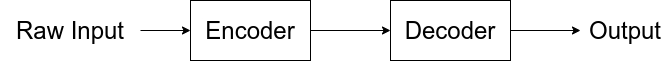
\includegraphics[width=\textwidth]{gambar/transformer_architecture.png}
    \caption{Model Arsitektur Transformer}
    \label{fig: architecture_transformer}
\end{figure}

Gambar \ref{fig: architecture_transformer} merupakan bentuk arsitektur dari Transformer. Bagian \textit{encoder} berisi metode \textit{self-attention} yang berguna untuk merubah token - token representasi dari teks menjadi memiliki nilai bias untuk digunakan pada proses selanjutnya. Sedangkan bagian \textit{decoder} merupakan bagian yang berfungsi untuk melakukan keluaran berdasarkan nilai bias tersebut.

\section{BERT}
BERT merupakan suatu model yang cukup baru dan merupakan singkatan dari \textit{\textbf{B}idirectional \textbf{E}ncode \textbf{R}epresentations from \textbf{T}ransformers}, adalah sebuah model bahasa yang sudah dilakukan proses \textit{pretrained} dengan menggunakan pendekatan \textit{fine-tuning}. BERT merupakan hasil penggabungan antara \textit{bi-directionality} dan \textit{transformer encoder}. \cite{devlin2019bert}

\begin{figure}[h]
    \begin{center}
        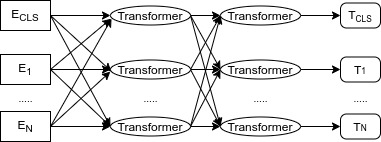
\includegraphics[width= .8\linewidth]{gambar/bert_archi_base.png}
        \caption{pendekatan dua arah BERT}
        \label{fig: bidirectionalBert}
    \end{center}
\end{figure}

Masukan dari BERT dapat berupa teks mentah dengan sedikit melakukan \textit{preprocessing} sebelumnya. Awalnya, BERT akan melakukan \textit{word embedding}, yaitu suatu metode untuk mendapatkan token dari kata yang dimasukkan berdasar pada kamus. Karena proses ini pulalah, terdapat beberapa versi BERT yang khusus untuk bahasa tertentu dan ada juga versi BERT untuk beberapa bahasa sekaligus. Setelah melakukan \textit{word embedding}, BERT akan memasukkan token \texttt{[CLS]}. Token tersebut digunakan sebagai representasi keseluruhan teks dan dapat digunakan sebagai basis dari proses klasifikasi. Selanjutnya, BERT akan membagi kalimat menggunakan token \texttt{[SEP]}. Dari token tersebut akan didapat \textit{segment embeddings} yang berfungsi untuk membedakan antara kalimat A dan kalimat B. \textit{Embedding} yang terakhir adalah berupa \textit{position embedding} yang digunakan untuk menunjukkan posisi kata dalam suatu kalimat. Gambar \ref{fig: bertToken} merupakan gambaran secara garis besar bagaimana BERT memahami suatu input.

\begin{figure}[h]
    \begin{center}
        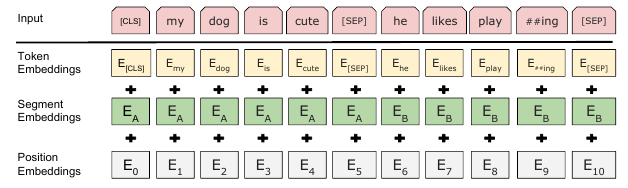
\includegraphics[width= 0.9\linewidth]{gambar/bert.png}
        \caption{Token dalam BERT \cite{devlin2019bert}}
        \label{fig: bertToken}
    \end{center}
\end{figure}

Keluaran dari BERT adalah berupa token - token yang merepresentasikan kalimat tersebut. Nantinya, token - token tersebut dapat digunakan sebagai masukan dari algoritma lain seperti misalnya CNN, maupun menggunakan isi token \texttt{[CLS]} sebagai masukan algoritma klasifikasi seperti \textit{Logistic Regression}.

Keuntungan dari penggunaan BERT adalah apabila dibandingkan dengan \textit{word2vec} yang juga sama - sama merubah kata - kata menjadi vektor atau token adalah, BERT tidak hanya merubah kata - kata tersebut menjadi token saja, namun juga melakukan relasi dan konteks \textit{learning} sehingga token dapat lebih menunjukkan konteks dari kalimat. Sebagai contoh, dalam kalimat "hadiah untuk ibuku sudah dikemas" dan kalimat "acara tersebut dikemas dengan rapi". Kata - kata "dikemas" disini memiliki 2 arti yang berbeda, yang pertama adalah berarti dibungkus, sedangkan yang kedua adalah ditampilkan. Apabila kita menggunakan \textit{word2vec} biasa, kata - kata "dikemas" akan memiliki token yang sama, sedangkan apabila menggunakan BERT, kata tersebut akan memiliki token yang berbeda. \cite{coenen2019visualizing}

Di Indonesia sendiri sudah terdapat beberapa model BERT yang khusus untuk bahasa Indonesia seperti model yang dibuat oleh Cahya dengan menggunakan gabungan dari 522 MB wikipedia Indonesia dan 1GB surat kabar Indonesia \cite{cahya_bert}, dan IndoBERT dengan 12 \textit{layer} dan dilatih menggunakan 31,923 kata dalam bahasa Indonesia \cite{koto2020indolem}. Hal ini kurang lebih sama dengan ukuran BERT-\textit{Base} yang juga memiliki 12 \textit{layer} dan 30,000 kata dalam bahasa Inggris \cite{devlin2019bert}.

\section{Metode Analisa Performa}
Terdapat beberapa metode yang bisa dilakukan untuk mengetahui apakah suatu model memiliki akurasi yang cukup. Penelitian ini menggunakan beberapa formula yang sudah ditentukan seperti \textit{recall, precision, f1-score} dan \textit{confusion matrix}.

\subsection{\textit{Recall}}

\textit{Recall} adalah formula yang harus digunakan ketika kita memiliki data yang tidak seimbang. Berbeda dengan akurasi yang hanya menghitung persentase model memprediksi hasil yang sesuai dengan label secara keseluruhan, \textit{recall} akan menghitung rasio nilai yang diprediksi positif dengan total keseluruhan nilai yang positif \cite{metrics_ml}. Rumus \ref{form:recall} merupakan rumus untuk menghitung \textit{recall}.

\begin{equation}
    Recall = \frac{TP}{TP+FN}
    \label{form:recall}
\end{equation}

\subsection{\textit{Precision}}

Seringnya, kita tidak hanya melihat tingkat akurasi suatu model hanya dengan besaran \textit{recall} maupun tingkat akurasi nya. \textit{Precision} adalah formula untuk menghitung rasio dari prediksi TP (\textit{True Positive}) yang benar dengan keseluruhan prediksi. Apabila prediksi yang dilakukan oleh model kita ternyata memiliki tingkat presisi yang tinggi namun memiliki tingkat \textit{recall} yang rendah, ada kemungkinan model tidak dapat melakukan prediksi pada data yang bersifat negatif \cite{metrics_ml}. Rumus \ref{form:precision} merupakan rumus untuk menghitung nilai dari \textit{precision} suatu model.

\begin{equation}
    Precision = \frac{TP}{TP+FP}
    \label{form:precision}
\end{equation}

Baik \textit{recall} maupun \textit{precision} merupakan nilai yang cukup penting terutama pada data yang tidak seimbang. Terdapat 3 kondisi yang umum terjadi pada saat membandingkan antara \textit{precision} dengan \textit{recall}.

\begin{itemize}
    \item \textit{Recall} tinggi, \textit{Precision} rendah

          Sebagian besar data positif dapat diprediksi dengan benar (\textit{False Negative} yang Rendah), namun hanya ada sebagian kecil data negatif yang diprediksi dengan benar (\textit{True Negative} rendah).

    \item \textit{Recall} rendah, \textit{Precision} tinggi

          Hasil prediksi model memiliki banyak sekali prediksi negatif (\textit{False Negative} tinggi), namun apabila digunakan untuk memprediksi data positif, maka hasil prediksi sebagian besarnya adalah benar (\textit{False Positive} rendah).

    \item \textit{Recall} tinggi, \textit{Precision} tinggi

          Merupakan hasil yang ideal dalam pembuatan model pembelajaran mesin. Disini didapatkan bahwa baik hasil prediksi untuk data positif maupun hasil prediksi untuk data negatif sebagian besarnya adalah benar (\textit{True Positive} dan \textit{True Negative} tinggi).

\end{itemize}

\subsection{\textit{F1-Score}}

\textit{F1-Score} adalah besaran yang berasal dari rata - rata harmonik dari \textit{recall} dan \textit{precision}. Rata  - rata harmonik dipilih karena akan menghasilkan nilai rata - rata yang lebih rendah dalam kondisi tidak seimbang apabila dibandingkan dengan rata - rata aritmatis biasa. Dengan rata - rata seperti itu, suatu model dapat menjadi lebih rentan terhadap bias dan memudahkan pada saat pembuatan model \cite{metrics_ml}. Rumus \ref{form: f1-score} merupakan rumus untuk menghitung f1-score.

\begin{equation}
    \label{form: f1-score}
    F1-Score = 2 \times \frac{\textit{Recall} \times \textit{Precision}}{\textit{Recall} + \textit{Precision}}
\end{equation}

\subsection{\textit{Confusion Matrix}}

\textit{Confusion Matrix} adalah tabel kesimpulan yang berisi jumlah prediksi baik yang benar maupun yang salah dan nilai label baik yang benar maupun salah. Biasanya tabel jenis ini digunakan untuk tugas yang bersifat klasifikasi dan berfungsi untuk memvisualisasi bagaimana suatu performa model dalam suatu dataset.

\begin{table}
    \caption{Contoh \textit{Confusion Matrix}}
    \label{tab:cth_confusion_mtrx}
    \centering
    \begin{tabular}{|l|l|l|l|l}
        \cline{1-4}
        \multicolumn{2}{|l|}{\multirow{2}{*}{}} & \multicolumn{2}{l|}{\textbf{Aktual}} &                \\ \cline{3-4}
        \multicolumn{2}{|l|}{}                  & Positif                              & Negatif &      \\ \cline{1-4}
        \multirow{2}{*}{\textbf{Prediksi}}      & Positif                              & TP      & FP & \\ \cline{2-4}
                                                & Negatif                              & FN      & TN & \\ \cline{1-4}
    \end{tabular}
\end{table}

Tabel \ref{tab:cth_confusion_mtrx} adalah contoh tabel \textit{confussion matrix} untuk prediksi dengan 2 label. Apabila melihat pada tabel tersebut, dapat terlihat bahwa jumlah prediksi dipecah menjadi masing - masing kelas. Diharapkan dengan dipecah menjadi beberapa kelas seperti itu, akan membuat proses pengujian lebih mudah karena akan lebih mudah melihat pada saat model memprediksi jenis data apa yang masih memiliki tingkat akurasi yang kurang bagus. Terdapat beberapa hal yang harus diketahui untuk dapat memahami sebuah tabel \textit{confussion matrix}, yaitu :

\begin{itemize}[nolistsep]
    \item Positif (P)

          Berisi data yang bernilai positif, baik data tersebut beasal dari hasil prediksi maupun data aktual yang didapat dari dataset.

    \item Negatif (N)

          Berisi data yang bernilai negatif, baik data tersebut berasal dari hasil prediksi maupun data aktual yang didapat dari dataset.

    \item \textit{True Positive} (TP)

          Suatu kondisi dimana baik hasil prediksi maupun data aktual sama - sama bernilai positif. Semakin tinggi nilai dari TP, semakin akurat pulalah model yang sudah dibuat.

    \item \textit{False Positive} (FP)

          Suatu kondisi dimana hasil prediksi adalah positif, namun pada data aktual bernilai negatif. Biasanya, semakin tinggi nilai dari FP ini, maka model semakin memilki kecenderungan untuk mengeluarkan nilai positif dibanding negatif atau terjadinya bias pada model.

    \item \textit{True Negative} (TN)

          Suatu kondisi dimana hasil prediksi dan data aktual bernilai negatif. Semakin tinggi nilai FN berarti semakin akurat model yang sudah dibuat.

    \item \textit{False Negative} (FN)

          Suatu kondisi dimana hasil prediksi adalah negatif, namun pada data aktual bernilai positif. Biasanya, semakin tinggi nilai dari TN ini, maka model semakin memiliki kecenderungan untuk mengeluarkan nilai negatif dibanding positif.


\end{itemize}

\cleardoublepage

% Bab 3 desain dan implementasi
\chapter{DESAIN DAN IMPLEMENTASI}
\label{chap:desainimplementasi}

% Ubah bagian-bagian berikut dengan isi dari desain dan implementasi
Penelitian ini dilaksanakan sesuai dengan desain sistem berikut dengan implementasinya. Desain sistem merupakan konsep dari pembuatan dan perancangan infrastruktur dan kemudian diwujudkan dalam bentuk blok-blok alur yang harus dikerjakan. Sedangkan untuk bagian implementasi merupakan pelaksanaan teknis untuk setiap blok pada desain sistem.

\begin{figure}[h!]
  \begin{center}
    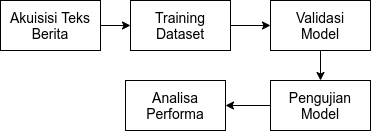
\includegraphics[width= 0.7\linewidth]{gambar/research_flow.png}
    \caption{bagan umum metodologi penelitian}
    \label{fig: base_method}
  \end{center}
\end{figure}

Gambar \ref{fig: base_method} merupakan bagan yang menunjukkan secara garis besar bagaimana proses implementasi model pada penelitian ini. Proses \textit{training} akan dilakukan beberapa kali dengan merubah parameter dari model untuk meningkatkan tingkat akurasi pada model akhir.

\section{Desain Sistem}

Tugas akhir ini adalah penelitian dalam bidang pemrosesan teks yang bertujuan untuk mendeteksi suatu berita hoaks berbahasa Indonesia secara otomatis berbasis \textit{Deep Learning}. Dalam proses \textit{training}-nya model ini akan menggunakan data yang dikumpulkan dari situs - situs berita yang sudah terverifikasi dan situs berita yang memang berisi berita palsu yang sudah ditemukan.


\section{Alur Kerja}

Terdapat beberapa langkah dalam melakukan implementasi dalam penelitian ini. Tahapan - tahapan ini sesuai berdasarkan dengan metodologi penelitian, yaitu :

\begin{enumerate}[nolistsep]
  \item Akuisisi Data
  \item \textit{Pre-Processing}
  \item Proses \textit{Training}
  \item Proses Pengujian
  \item Analisa Performa
\end{enumerate}

Berdasarkan bagan pada gambar \ref{fig: base_method}, proses yang pertama kali dilakukan adalah proses akuisisi data. Data yang diambil adalah data berupa berita yang berasal dari situs yang sudah terverifikasi seperti \url{liputan6.com}, \url{detik.com}, dan sebagainya. Selain itu, kami juga mengambil data berupa berita palsu yang sudah dipastikan sebagai palsu yang berasal dari situs seperti \url{turnbackhoax.com}. Tujuan dari proses akuisisi data ini adalah karena hampir tidak ada set data yang cukup banyak yang dapat digunakan sebagai data untuk proses klasifikasi berita palsu. Pada proses akuisisi ini juga dilakukan proses memberi label kepada kumpulan data dengan melihat tautan sumber berita.

Setelah set data berhasil didapatkan, proses selanjutnya adalah \textit{training} dimana data akan dimasukkan ke dalam model yang menggunakan metode berbasis \textit{Transformer} yaitu \textit{\textbf{B}idirectional \textbf{E}ncode \textbf{R}epresentations from \textbf{T}ransformers}(BERT).

\section{Akuisisi Data}

Pada tahap akuisisi data, data diambil dari situs - situs berita berbahasa Indonesia yang beredar di internet. Data - data tersebut akan diambil menggunakan metode \textit{webcrawling} sehingga diharapkan, apabila suatu saat diperlukan data dengan jumlah yang lebih banyak dapat dengan mudah memanggil program \textit{webcrawling} yang sudah dibuat. Untuk saat ini, keseluruhan kode program dapat diakses dan diunduh pada tautan \url{https://github.com/chillytaka/berita-crawler}.

\subsection{Sumber Akuisisi Data}

Sebagai dasar awal dari dataset, kami menggunakan dataset yang bersumber dari situs \url{https://data.mendeley.com/datasets/p3hfgr5j3m/1}. Namun, karena jumlah data dari situs tersebut dinilai kurang memadai untuk penelitian ini (data dari sumber tersebut hanya berjumlah 600 data), kami memutuskan untuk menambah dataset lagi menggunakan teknologi \textit{webcrawling}.

Sumber data yang pertama diambil berasal dari beberapa situs berita yang sudah terverifikasi seperti \url{liputan6.com}, \url{detik.com}, \url{kompas.com}, \url{cnnindonesia.com}. Sumber - sumber berita terverifikasi ini dipilih untuk menghilangkan proses pemberian label setelah dataset terkumpul. Diharapkan dengan mengambil teks berita dari situs yang sudah terpercaya dapat membuat model mengetahui bagaimana teks suatu berita yang berasal dari sumber terverifikasi. Selain itu, untuk lebih mengerucutkan lagi, kami hanya mengambil berita yang membahas isu nasional dan tidak mengambil berita yang membahas olahraga, opini, maupun jenis tipe berita lainnya. Gambar \ref{fig: news_source} menunjukkan salah satu situs berita yang digunakan dalam pengambilan dataset penelitian ini.

\begin{figure}[h!]
  \begin{center}
    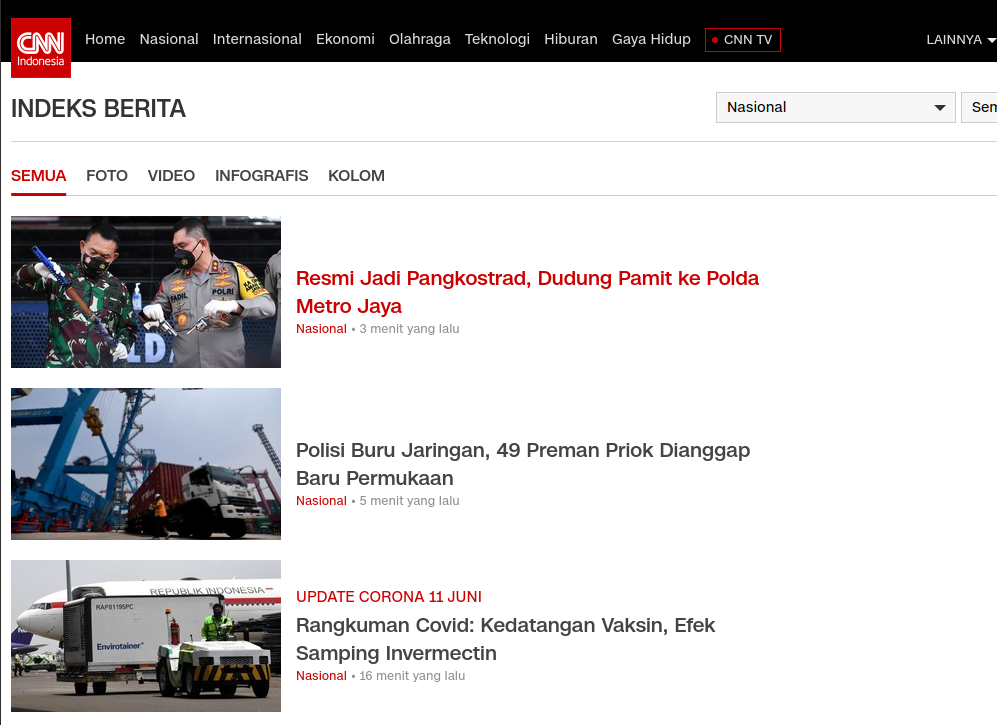
\includegraphics[width= .9\linewidth]{gambar/cnn_news.png}
    \caption{contoh situs sumber berita terverifikasi}
    \label{fig: news_source}
  \end{center}
\end{figure}

Sedangkan sumber kedua yang digunakan untuk proses pengambilan data pada penelitian ini adalah situs \url{turnbackhoax.id}. Situs tersebut adalah situs khusus yang mengumpulkan berita - berita yang sudah dipastikan palsu yang berasal dari berbagai sumber. Selain itu, situs ini juga mengambil data dari hasil unggahan masyarakat Indonesia sendiri melalui sosial media dan grup resmi \url{turnbackhoax.id}. Keuntungan dari metode seperti ini adalah sebuah unggahan akan dicek berkali - kali oleh anggota grup sehingga mengurangi kemungkinan terdapat berita yang salah klasifikasi. Alasan lain situs ini dipilih sebagai sumber adalah adanya format yang kurang lebih sama antara setiap unggahan sehingga akan memudahkan dalam proses pengambilan teks berita.

\begin{figure}[h!]
  \begin{center}
    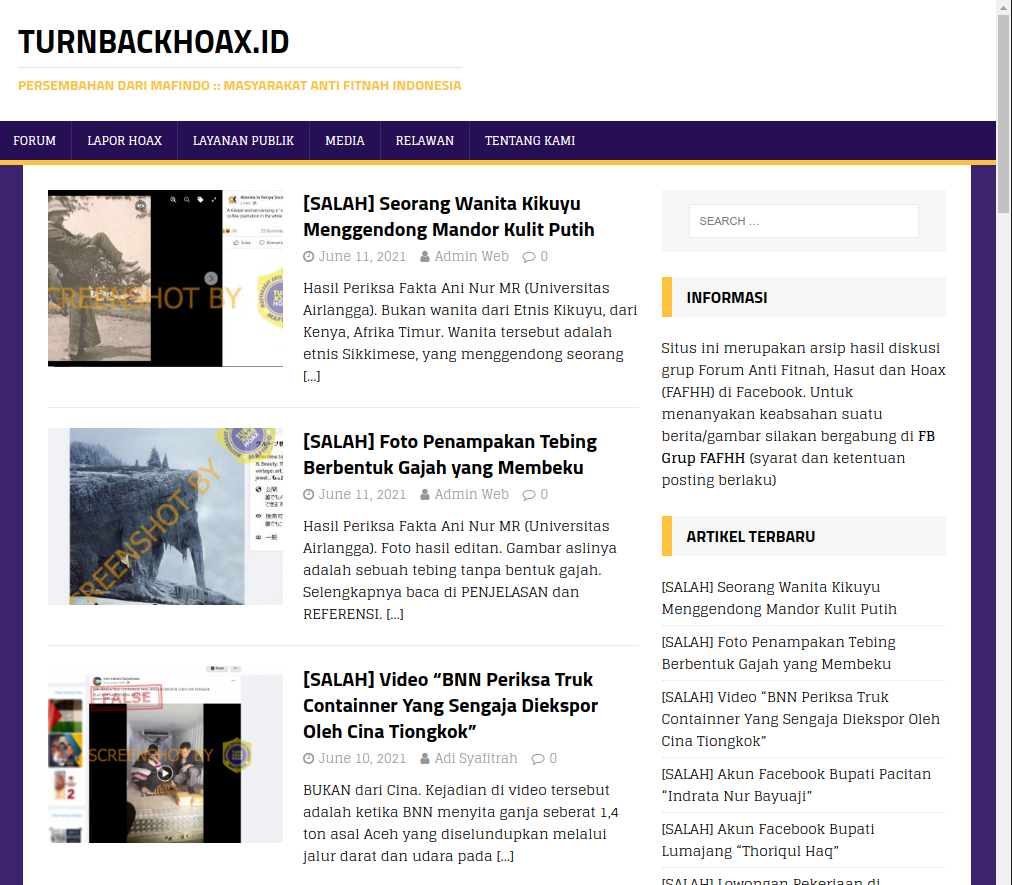
\includegraphics[width= \linewidth]{gambar/hoax_news.png}
    \caption{contoh situs sumber berita palsu}
    \label{fig: hoax_news_source}
  \end{center}
\end{figure}

\subsection{Proses Akuisisi Data}

Setelah menentukan situs - situs untuk digunakan sebagai sumber berita, langkah selanjutnya adalah memulai proses akuisisi data. Disini, hal yang paling pertama kali dilakukan adalah mengambil kode sumber dari situs - situs tersebut. Hal ini dilakukan guna mempermudah saat melakukan penyaringan untuk mendapatkan teks berita. Gambar \ref{fig:webcrawl_method} adalah gambaran garis besar yang kami lakukan dalam program \textit{web crawl} kami. Dimulai dengan memasukkan kode HTML mentah, kemudian merubah kode mentah tersebut menjadi objek yang lebih mudah untuk dilakukan pemrosesan dalam python, mengambil teks berita dan melakukan pembersihan terhadap teks tersebut, terakhir menghasilkan keluaran berupa file .CSV dengan format yang sesuai.

\begin{figure} [ht]
  \centering
  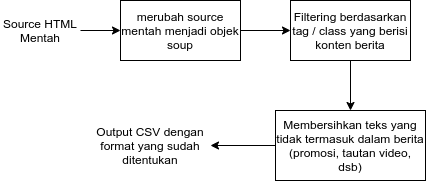
\includegraphics[width=.9\linewidth]{gambar/webcrawl method_box.png}
  \caption{Garis besar alur program \textit{web crawl}.}
  \label{fig:webcrawl_method}
\end{figure}

\begin{figure}[h!]
  \begin{lstlisting}[
    language=HTML, 
    caption={Penggalan Kode Sumber HTML \url{detik.com}.},
    label={lst:source_detik}
]

...
<div class="detail__body itp_bodycontent_wrapper">
<div class="detail__body-text itp_bodycontent">

<strong>Jakarta</strong> - Koalisi <a href="https://
detik.com/tag/jokowi" target="_blank">Jokowi</a> 
sedang menyusun visi-misi jagoannya. Setelah 
menerima masukan dari <a href="https://detik.com/
tag/muhammadiyah" target="_blank"> Muhammadiyah</a>,
 ... 
Dan kita pun membuka diri untuk menerima 
masukan untuk penyempurnaan," imbuhnya.<br><br><!--
s:parallaxindetail--><div class="clearfix"></div><style>
...

\end{lstlisting}
\end{figure}

\textit{Library} yang kami gunakan untuk melakukan \textit{crawling} adalah \textit{BeautifulSoup}, sebuah \textit{library} yang akan secara otomatis merubah dari suatu teks HTML menjadi objek \textit{soup} yang lebih mudah untuk dilakukan pemrosesan di dalam python.

Yang pertama kali harus kami lakukan adalah menentukan \textit{tag} atau \textit{class} HTML yang akan digunakan sebagai masukan pada program guna melakukan penyaringan terlebih dahulu. Apabila merujuk pada listing \ref{lst:source_detik} \textit{class} yang berisi teks seluruh berita adalah \texttt{detail\_\_body\-text} sehingga kami melakukan penyaringan dengan memasukkan \textit{class} tersebut ke dalam parameter.

Namun, walaupun sudah melakukan penyaringan, masih terdapat beberapa teks yang tidak diperlukan. Biasanya, teks - teks tersebut masuk ke dalam  kategori seperti catatan dari penulis, iklan, dan tautan untuk menuju ke berita yang masih berhubungan. Sehingga, setelah melakukan penyaringan, masih diperlukan lagi pembersihan isi berita dari teks - teks yang tidak diperlukan.

Terakhir, adalah melakukan keluaran berupa \textit{file} .CSV. Alasan menggunakan format CSV sebagai keluaran adalah karena format tersebut bersifat 'terbuka' dan dapat dibuka oleh berbagai \textit{software} spreadsheet pada umumnya, selain itu akan lebih mudah memproses data dalam bentuk .CSV di python dibandingkan dengan format lainnya.

Untuk memudahkan penggunaan perangkat lunak \textit{webcrawler} yang kami buat, kami menggunakan berkas dengan format .json untuk mengatur sumber, banyak berita dan filter tanggal yang nantinya akan dibaca oleh program dan mengambil berita dengan parameter tersebut. Tabel \ref{tab:contoh_dataset} merupakan contoh hasil keluaran dari program \textit{webcrawling} yang digunakan.

\begin{table}
  \caption{Contoh Dataset}
  \label{tab:contoh_dataset}
  \centering
  \begin{tabular}{ | p{.7\linewidth} | l | }
    \hline
    \textbf{berita}                                                                                                                                                                                                                   & \textbf{\textit{tagging}} \\ \hline
    Wakil Gubernur DKI Jakarta Sandiaga Uno menargetkan pengerjaan tahap awal Stadion BMW dilakukan pada Oktober. Stadion ini diperuntukkan bagi klub Persija....                                                                     & Valid                     \\ \hline
    "Komisi II bersama KPU dan Bawaslu masih membahas ketentuan wajib cuti bagi petahana presiden yang maju Pilpres 2019. Mekanisme pengambilan.....                                                                                  & Valid                     \\ \hline
    Jaksa penuntut Ulumum (JPU) pada Komisi Pemberantasan Korupsi (KPK) mencecar Pejabat Pembuat Komitmen (PPK) reguler pada Direktorat Perlindungan Sosial Korban Bencana Sosial Kemensos Victorious Saut Hamonangan Siahaan soal... & Valid                     \\ \hline
    “Halo Kak! Aku Winda Dari Team Giveaway BAIM WONG Anda Memenangkan Hadiah Uang 100Jt dari kami info klik: https://wa.me/+6285796306857”                                                                                           & Hoax                      \\ \hline
    “Apa yang terjadi dengan hewan dalam penelitian?   Teknologi ini telah dicoba pada hewan, dan pada hewan penelitian yang dilakukan, semua hewan mati , tidak langsung dari suntikan...                                            & Hoax                      \\ \hline
    “Kadrun istilah dr PKI alias KOMUNIS ditujukan buat islam. Kl mau jd komunis pake aja istilah kadrun buat umat islam. Auto lsg Komunis”                                                                                           & Hoax                      \\ \hline
  \end{tabular}
\end{table}

Setelah melakukan penggabungan antara data yang berasal dari \url{https://data.mendeley.com/datasets/p3hfgr5j3m/1} dengan dataset hasil dari proses \textit{webcrawling}, maka didapatkan total data sebesar 1621 data dengan pola penyebaran data yang kurang lebih seimbang sehingga mengurangi kemungkinan terjadinya bias pada saat proses melatih model. Tabel \ref{tab:dataset} menunjukkan secara lebih detail berapa banyak distribusi  data yang berada di dalam dataset yang digunakan dalam penelitian ini.

\begin{table}
  \caption{Jumlah Dataset yang digunakan}
  \label{tab:dataset}
  \centering
  \begin{tabular}{ | l | l | }
    \hline
    \textbf{Label} & \textbf{Jumlah Data} \\ \hline
    \textit{Hoaks} & 885                  \\ \hline
    \textit{Valid} & 736                  \\ \hline
    \textbf{Total} & \textbf{1621}        \\ \hline
  \end{tabular}
\end{table}

\section{\textit{Preprocessing}}

\begin{figure}[h!]
  \begin{center}
    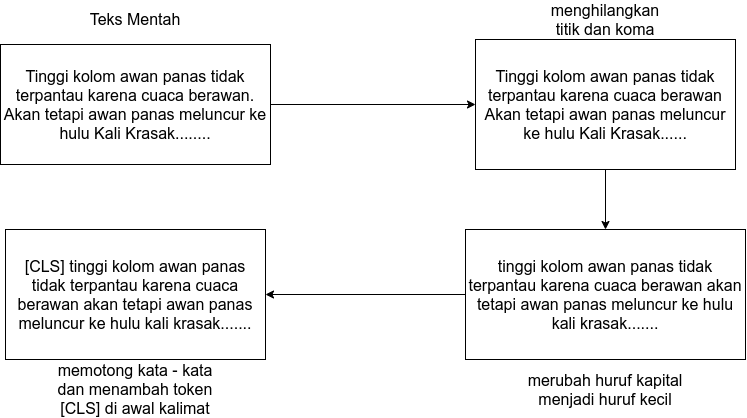
\includegraphics[width= \linewidth]{gambar/preprocess.png}
    \caption{Metode Preprocessing}
    \label{fig: metodologi_preprocessing}
  \end{center}
\end{figure}

Pada proses ini, data akan disiapkan terlebih dahulu agar dapat diproses oleh BERT. Proses penyiapan data meliputi menghilangkan titik dan koma, dan merubah huruf kapital yang ada menjadi huruf kecil seluruhnya. Dan karena BERT memiliki maksimal kata - kata yang dapat diproses dalam sekali waktu sejumlah 512 kata atau token, maka harus dilakukan penyingkatan teks, dapat dengan cara melakukan pengambilan 512 karakter pertama, terakhir maupun gabungan dari kedua bentuk. Chi Sun et al. menemukan bahwa mengambil teks dengan cara mengambil bagian tengah sebanyak 128 kata pertama dan mengambil sebanyak 382 kata pada bagian akhir menghasilkan hasil akurasi yang lebih baik dalam beberapa tugas \cite{sun2019fine}. Langkah terakhir adalah menambahkan token \texttt{[CLS]} di awal kalimat. Untuk lebih jelasnya, bisa melihat pada Gambar \ref{fig: metodologi_preprocessing}.

Selain itu, juga akan dilakukan pembagian dataset yang awalnya berjumlah 1621 akan dibagi menjadi 3 bagian dengan ketentuan 70\% akan digunakan pada saat proses \textit{training}, 10\% akan digunakan untuk proses validasi, dan sisanya sebesar 20\% akan digunakan pada saat pengujian.

\begin{enumerate}
  \item \textit{Training}

        Set ini digunakan oleh algoritma BERT sebagai masukan saat melakukan proses \textit{training} sehingga akan didapat model yang sesuai.

  \item Validasi

        Set ini digunakan pada saat selesai melakukan validasi model setelah melakukan \textit{training}. Digunakan untuk menentukan apakah suatu model sudah memiliki \textit{weight} yang sesuai ataukah masih perlu melakukan \textit{training} lagi. Selain itu, set ini juga digunakan untuk menghindari kemungkinan \textit{overfitting} maupun \textit{underfitting} dalam model.

  \item Pengujian

        Set yang digunakan untuk melakukan pengujian akurasi model setelah proses \textit{training} dan validasi selesai. Hasil akurasi dari pengujian inilah yang akan digunakan sebagai hasil dari model.

\end{enumerate}

Untuk lebih jelasnya, silahkan lihat tabel \ref{tab:dataset_section}. Dari tabel tersebut dapat dilihat bahwa pembagian dan total dari dataset sudah sesuai.

\begin{table}
  \caption{Rincian Pembagian Dataset}
  \label{tab:dataset_section}
  \centering
  \begin{tabular}{ | l | l | l | l | }
    \hline
    \textbf{Bagian}                      & \textbf{Hoaks} & \textbf{Valid} & \textbf{Total Data} \\ \hline
    \textit{Training}                    & 647            & 519            & 1166                \\ \hline
    \textit{Validasi}                    & 85             & 78             & 163                 \\ \hline
    \textit{Pegujian}                    & 153            & 139            & 292                 \\ \hline
    \multicolumn{3}{|l|}{\textbf{Total}} & \textbf{1621}                                         \\ \hline
  \end{tabular}
\end{table}

\section {Proses \textit{Training}}

\begin{figure}[h!]
  \begin{center}
    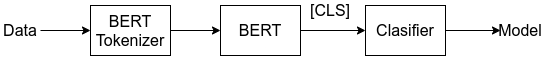
\includegraphics[width= 0.9\linewidth]{gambar/training.png}
    \caption{Metode Training}
    \label{fig: metodologi_training}
  \end{center}
\end{figure}

Pada tahap ini, teks yang sudah melewati proses \textit{preprocessing} akan dilakukan proses Tokenizer. Tokenizer adalah proses untuk merubah kata - kata dalam teks menjadi token sesuai dengan \textit{word embedding} yang sudah ada pada \textit{pretrained} BERT. Barulah pada saat itu, BERT dapat melakukan \textit{training} berdasarkan data dari \textit{dataset}.

Keluaran dari BERT akan diambil isi token \texttt{[CLS]}-nya dan dimasukkan kedalam algoritma klasifikasi, dalam penelitian ini kami memilih untuk menggunakan metode \textit{Linear Regression}. \textit{Linear Regression} digunakan sebagai algoritma klasifikasi yang cukup mudah namun memiliki tingkat akurasi yang cukup. Gambar \ref{fig: metodologi_training} dapat digunakan sebagai penjelas.

Pada tahap ini juga dilakukan pengaturan ukuran \textit{batch}, \textit{learning rate} dan juga \textit{epoch}. \textit{Batch} adalah banyaknya teks yang diproses untuk setiap iterasi, semakin tinggi nilai \textit{batch} yang dikonfigurasi, maka proses \textit{training} akan semakin cepat namun memakan memori yang lebih banyak. Berhubung algoritma BERT adalah algoritma yang cukup berat karena memiliki \textit{layer} yang cukup banyak, dan karena terdapat keterbatasan \textit{resource} maka dalam penelitian ini kami menggunakan \textit{batch} dengan nilai 8.

\textit{Epoch} adalah berapa banyak suatu algoritma melakukan proses \textit{training} dan validasi sebelum dianggap final. Disini \textit{epoch} harus diperhatikan agar jumlah \textit{loss} yang terjadi pada saat proses \textit{training} tidak terlalu tinggi karena merupakan ciri - ciri \textit{underfitting} namun juga tidak terlalu rendah selama beberapa \textit{epoch} untuk menghindari kemungkinan \textit{overfitting}. Berhubung kami hanya menggunakan BERT untuk memproses teks yang relatif lebih mudah, kami hanya menggunakan \textit{epoch} sebesar 10.

\textit{learning rate} adalah seberapa banyak \textit{hyperparameter} yang dirubah selama proses \textit{training}. \textit{hyperparameter} digunakan untuk merubah \textit{weight} selama proses \textit{training} berdasarkan \textit{feedback} saat proses validasi. Disini kami menggunakan nilai yang direkomendasikan oleh pembuat model BERT yang kami gunakan, yaitu 0.000002 \cite{koto2020indolem}.

\begin{table}
  \caption{Konfigurasi pada BERT}
  \label{tab:bert_config}
  \centering
  \begin{tabular}{ | l | l | }
    \hline
    \textbf{Jenis Konfigurasi} & \textbf{Keterangan} \\ \hline
    \textit{batch}             & 8                   \\ \hline
    \textit{learning rates}    & 2e-6                \\ \hline
    \textit{epoch}             & 5                   \\ \hline
  \end{tabular}
\end{table}


\section{Proses Pengujian}

Proses pengujian dalam penelitian ini dibagi menjadi 2 bagian, bagian yang pertama dilakukan pada saat model selesai melakukan proses \textit{training} namun masih memiliki iterasi \textit{epoch} yang belum selesai. Proses ini bernama validasi. Proses ini sangat vital karena dengan validasi kita dapat mengetahui apakah model kita mengalami \textit{overfitting} maupun \textit{underfitting}. Salah satu ciri yang paling mudah yang menandakan kemungkinan terjadinya \textit{overfitting} adalah ketika besaran \textit{training loss} suatu model menjadi semakin kecil, namun besaran \textit{validation loss}-nya malah semakin besar di setiap iterasi. Sedangkan \textit{underfitting} terjadi ketika baik \textit{training loss} maupun \textit{validation loss} memiliki nilai yang terlalu besar. Selain itu pada proses validasi ini, data yang digunakan adalah data yang sama sekali baru dan tidak digunakan selama proses \textit{training} guna menghindari kemungkinan terjadinya bias yang biasa terjadi apabila suatu model diuji pada data yang sama yang digunakan pada saat proses \textit{training}. Berdasarkan data pada proses validasi, algoritma \textit{optimizer} akan memutuskan untuk merubah \textit{weight} dalam \textit{hidden node} BERT sehingga semakin mendekati titk akurasi tertingginya.

Bagian selanjutnya dari proses pengujian adalah melakukan \textit{test}. Sama seperti pada waktu proses validasi, dataset yang digunakan juga sama sekali berbeda dengan data yang digunakan pada waktu \textit{training} maupun pada waktu \textit{validasi}. Dari proses ini, dapat diambil kesimpulan apakah suatu model tersebut dapat dilakukan perbaikan lagi denga cara \textit{re-training} dan merubah beberapa parameter maupun konfigurasi yang sudah diatur pada saat proses \textit{training}, ataukah model tersebut dirasa sudah cukup baik dan akan melanjutkan ke proses berikutnya.
\cleardoublepage

% Bab 4 pengujian dan analisis
\chapter{PENGUJIAN DAN ANALISIS}
\label{chap:pengujiananalisis}

% Ubah bagian-bagian berikut dengan isi dari pengujian dan analisis
Pada penelitian ini dipaparkan hasil pengujian serta analisis yang dilakukan sesuai dengan desain sistem yang sudah dirancang pada bab sebelumnya. Dataset yang digunakan berasal dari \url{data.mendeley.com} ditambah dengan dataset yang berasal dari proses \textit{webcrawling} sendiri. Pengujian dilakukan dengan beberapa bagian sebagai berikut :

\begin{enumerate}[nolistsep]
    \item Pengujian Performa berdasar pada Penggalan Kata yang Diambil
    \item Pengujian Performa berdasarkan model BERT yang digunakan
    \item Pengujian Performa berdasarkan Pendekatan Cara \textit{Training}.
\end{enumerate}

Pada pengujian, masing - masing model menggunakan Google Collab dengan spesifikasi \textit{hardware} seperti yang dilampirkan pada tabel \ref{tab:specs_collab}

\begin{table}
    \caption{spesifikasi PC yang digunakan}
    \label{tab:specs_collab}
    \centering
    \begin{tabular}{|l|l|}
        \hline
        \textbf{Prosessor}            & 2 v-core Intel(R) Xeon(R) CPU @ 2.20GHz   \\ \hline
        \textbf{RAM}                  & Virtual Memory : 12GB                     \\ \hline
        \textit{\textbf{Storage}}     & SSD : 69GB                                \\ \hline
        \multirow{2}{*}{\textbf{GPU}} & Nvidia Tesla T4 16GB                      \\ \cline{2-2}
                                      & Nvidia K80 12GB                           \\ \hline
        \textbf{Sistem Operasi}       & Ubuntu 18.04.5 LTS (Bionic Beaver) 64-bit \\ \hline
    \end{tabular}
\end{table}

\section{Pengujian Performa berdasar pada Penggalan Kata yang Diambil}

Untuk saat ini, BERT hanya dapat memproses sebanyak 512 token sekaligus. Sehingga, untuk melakukan pemprosesan pada data dengan teks yang panjang, diperlukan pemotongan teks agar panjang teks menjadi sesuai.

Pengujian performa berdasar pada penggalan kata yang diambil ini bertujuan untuk mengetahui tingkat akurasi model BERT pada teks dengan cara pemotongan yang berbeda. Pembedaan ini dilakukan berdasarkan pada adanya berita yang menuliskan kesimpulan di awal, atau bisa juga menuliskan kesimpulan di akhir. Alternatif lain adalah mengambil sebagian teks di bagian awal dan mengambil sisanya di bagian akhir. Maka dari itu, dalam pengujian performa ini dilakukan dengan membagi teks pada beberapa cara memenggal kata, antara lain :

\begin{enumerate}[nolistsep]
    \item Mengambil bagian awal teks.
    \item Mengambil bagian akhir teks.
    \item Mengambil 129 token dari bagian awal teks dan 383 token dari bagian akhir teks.
\end{enumerate}

Dari total data yang berjumlah 1621 data, akan diambil 18\% nya sebagai dataset pengujian, sehingga berjumlah 292 dataset sebagai pengujian. Parameter pada pengujian untuk \textit{training} di atur agar sama untuk setiap pengujian, \textit{epoch} sebesar 7, \textit{leearning rate} sebesar 2e-5, dan \textit{epsilon} sebesar 1e-8, hal yang sama juga dilakukan pada model, pengujian ini menggunakan model BERT yang telah di-\textit{pre-trained} oleh Indobert. Untuk lebih jelasnya, silahkan lihat Tabel \ref{tab: truncate_param} yang berisi rincian parameter dan model yang digunakan untuk proses \textit{training}.

\begin{table}
    \caption{Konfigurasi Parameter Untuk Pengujian berdasarkan Pemotongan Kata}
    \label{tab: truncate_param}
    \centering
    \begin{tabular}{|l|l|}
        \hline
        \textit{\textbf{epoch}}          & 3                              \\ \hline
        \textit{\textbf{learning rates}} & 2e-5                           \\ \hline
        \textit{\textbf{epsilon}}        & 1e-4                           \\ \hline
        \textbf{model}                   & indobenchmark/indobert-base-p1 \\ \hline
    \end{tabular}
\end{table}

Keluaran dari model akan dibandingkan dengan label pada dataset, yang kemudian akan dihitung untuk menghasilkan \textit{confusion matrix}, \textit{recall, precision, accuracy} dan \textit{f1-score} sesuai dengan rumus yang telah dijelaskan pada bab tinjauan pustaka.

\subsection{Pengujian dengan Mengambil Bagian Awal Teks}

Terdapat beberapa ciri - ciri yang terdapat pada kebanyakan teks berita berbahasa Indonesia, salah satu dari ciri - ciri tersebut adalah menuliskan ringkasan berita pada paragraf awal kalimat. Format seperti ini biasanya cukup sering ditemui terutama pada berita yang memanfaatkan fitur halaman pada teks beritanya. Karenanya, pada jenis - jenis berita seperti ini, orang hanya perlu melihat beberapa kalimat awal untuk mengetahui apakah bahwa berita tersebut valid dan dapat dipercaya.

Seperti bisa dilihat pada tabel \ref{tab: const_awal}, dengan memotong teks berita pada bagian awal, didapatkan tingkat akurasi sebesar 89\% dengan nilai \textit{recall, precision, f1-score} kurang lebih sama. Selain itu, dapat dilihat juga pada kolom \textit{confusion matrix}, model yang sudah dibuat memiliki nilai FP dan FN yang sudah cukup sedikit. Namun, apabila melihat pada gambar \ref{fig: loss_const_awal}, terlihat bahwa model agak sedikit \textit{overfit}, sehingga terdapat kemungkinan akan memiliki tingkat akurasi yang lebih rendah pada saat implementasi.

\begin{table}
    \caption{Hasil Pengujian dengan Mengambil Awal Teks}
    \label{tab: const_awal}
    \centering
    \begin{tabular}{|l|l|l|}
        \hline
        \multicolumn{2}{|l|}{\textbf{Hasil Model}} & \textbf{Nilai}        \\ \hline
        \multirow{4}{*}{\textit{Confusion Matrix}} & TP             & 122  \\ \cline{2-3}
                                                   & FP             & 16   \\ \cline{2-3}
                                                   & TN             & 137  \\ \cline{2-3}
                                                   & FN             & 17   \\ \hline
        \multirow{2}{*}{\textit{Recall}}           & Hoax           & 89\% \\ \cline{2-3}
                                                   & Valid          & 88\% \\ \hline
        \multirow{2}{*}{\textit{Precision}}        & Hoax           & 90\% \\ \cline{2-3}
                                                   & Valid          & 88\% \\ \hline
        \multirow{2}{*}{\textit{F1-Score}}         & Hoax           & 89\% \\ \cline{2-3}
                                                   & Valid          & 88\% \\ \hline
        \multicolumn{2}{|l|}{\textit{Accuracy}}    & 89\%                  \\ \hline
    \end{tabular}
\end{table}

\begin{figure}[h]
    \begin{center}
        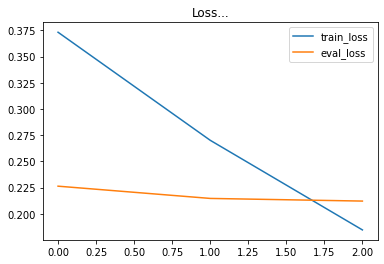
\includegraphics[width= 0.9\linewidth]{gambar/loss_concat_awal.png}
        \caption{Nilai \textit{Loss} saat Pengujian dengan Mengambil Bagian Awal Teks}
        \label{fig: loss_const_awal}
    \end{center}
\end{figure}


\subsection{Pengujian dengan Mengambil Bagian Akhir Teks}

Mirip seperti pengujian dengan mengambil bagian awal teks, terdapat ciri - ciri lain yang biasanya terdapat pada teks berita berbahasa Indonesia adalah adanya kesimpulan pada bagian akhir teks berita. Sehingga, setelah isi berita yang biasanya dibahas cukup dalam, pembaca dapat mengetahui bagaimana dan apa hubungan setiap informasi yang disajikan dengan peristiwa yang sedang dibahas dalam berita.

Dapat dilihat pada tabel \ref{tab: const_akhir}, model dengan cara memotong teks seperti ini berhasil mendapatkan tingkat akurasi sebesar 86\%. Namun, apabila melihat nilai \textit{recall} dan \textit{precision}-nya, ada indikasi bias dimana model lebih memiliki kecenderungan untuk mengeluarkan hasil hoaks bahkan pada berita valid sekalipun. Sedangkan, apabila melihat pada gambar \ref{fig: loss_const_akhir}, dapat dilihat bahwa baik nilai \textit{train loss} dan \textit{validation loss} sudah berada di titik optimal dan apabila dilakukan \textit{training} tambahan, akan membuat model \textit{overfit}.

\begin{table}
    \caption{Hasil Pengujian dengan Mengambil Akhir Teks}
    \label{tab: const_akhir}
    \centering
    \begin{tabular}{|l|l|l|}
        \hline
        \multicolumn{2}{|l|}{\textbf{Hasil Model}} & \textbf{Nilai}        \\ \hline
        \multirow{4}{*}{\textit{Confusion Matrix}} & TP             & 121  \\ \cline{2-3}
                                                   & FP             & 23   \\ \cline{2-3}
                                                   & TN             & 130  \\ \cline{2-3}
                                                   & FN             & 18   \\ \hline
        \multirow{2}{*}{\textit{Recall}}           & Hoax           & 88\% \\ \cline{2-3}
                                                   & Valid          & 84\% \\ \hline
        \multirow{2}{*}{\textit{Precision}}        & Hoax           & 85\% \\ \cline{2-3}
                                                   & Valid          & 87\% \\ \hline
        \multirow{2}{*}{\textit{F1-Score}}         & Hoax           & 86\% \\ \cline{2-3}
                                                   & Valid          & 86\% \\ \hline
        \multicolumn{2}{|l|}{\textit{Accuracy}}    & 86\%                  \\ \hline
    \end{tabular}
\end{table}

\begin{figure}[h]
    \begin{center}
        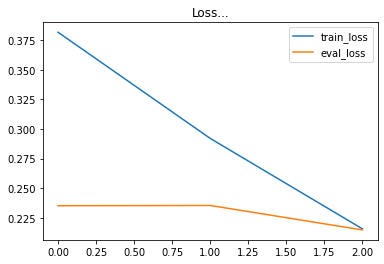
\includegraphics[width= 0.9\linewidth]{gambar/loss_concat_akhir.png}
        \caption{Nilai \textit{Loss} saat Pengujian dengan Mengambil Bagian Akhir Teks}
        \label{fig: loss_const_akhir}
    \end{center}
\end{figure}

\subsection{Pengujian dengan Mengambil Bagian Awal dan Akhir Teks}

Pengujian ini berdasarkan pada penelitian Chi Sun et al. yang menemukan bahwa dengan strategi pengambilan teks yang dibagi dua seperti ini akan dapat memberikan nilai akurasi yang lebih baik apabila dibandingkan dengan mengambil hanya di bagian awal maupun di bagian akhir saja \cite{sun2019fine}. Alasan dari penyebab lebih tingginya akurasi adalah karena dengan mengambil sebagian di awal maka sebagian dari ringkasan berita akan didapatkan, sedangkan mengambil sebagian di akhir adalah agar kesimpulan berita juga masuk ke dalam proses \textit{training}. Namun, pengujian tersebut dilakukan pada dataset teks berita berbahasa Inggris sehingga masih harus dilakukan pengujian lagi pada dataset teks berita berbahasa Indonesia.

\begin{table}[]
    \caption{Hasil Pengujian dengan Mengambil Tengah Teks}
    \label{tab: const_tengah}
    \centering
    \begin{tabular}{|l|l|l|}
        \hline
        \multicolumn{2}{|l|}{\textbf{Hasil Model}} & \textbf{Nilai}        \\ \hline
        \multirow{4}{*}{\textit{Confusion Matrix}} & TP             & 120  \\ \cline{2-3}
                                                   & FP             & 19   \\ \cline{2-3}
                                                   & TN             & 134  \\ \cline{2-3}
                                                   & FN             & 19   \\ \hline
        \multirow{2}{*}{\textit{Recall}}           & Hoax           & 88\% \\ \cline{2-3}
                                                   & Valid          & 86\% \\ \hline
        \multirow{2}{*}{\textit{Precision}}        & Hoax           & 88\% \\ \cline{2-3}
                                                   & Valid          & 86\% \\ \hline
        \multirow{2}{*}{\textit{F1-Score}}         & Hoax           & 88\% \\ \cline{2-3}
                                                   & Valid          & 86\% \\ \hline
        \multicolumn{2}{|l|}{\textit{Accuracy}}    & 87\%                  \\ \hline
    \end{tabular}
\end{table}

\begin{figure}[h]
    \begin{center}
        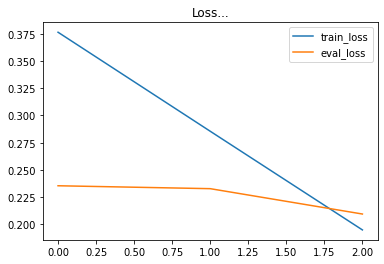
\includegraphics[width= 0.9\linewidth]{gambar/loss_concat_tengah.png}
        \caption{Nilai \textit{Loss} saat Pengujian dengan Mengambil Bagian Tengah Teks}
        \label{fig: loss_const_tengah}
    \end{center}
\end{figure}


\section{Pengujian Performa berdasarkan model BERT yang digunakan}

Terdapat banyak sekali model BERT yang sudah dibuat oleh berbagai orang di internet, ada model yang memiliki kemampuan \textit{multilanguage} sehingga bisa digunakan di berbagai bahasa sekaligus, namun kebanyakan model yang beredar adalah model yang menggunakan bahasa yang spesifik. Hal ini karena waktu \textit{pre-training} yang lebih singkat karena dataset yang lebih sedikit apabila dibandingkan model dengan kemampuan \textit{multilanguage} dan karena waktu \textit{pre-training} lebih sedikit, maka sumber daya yang digunakan juga menjadi lebih sedikit. Selain itu, dan hal ini adalah yang paling penting, hasil akurasi dari model yang hanya menggunakan 1 bahasa memiliki tingkat akurasi yang lebih tinggi apabila dibandingkan dengan model dengan banyak bahasa sekaligus.

Untuk model BERT yang menggunakan hanya bahasa Indonesia, terdapat 2 model yang bisa ditemukan pada waktu buku ini ditulis. Yang pertama dibuat oleh Bryan Wilie et al., sebagai bagian dari pengujian \textit{benchmark} berbahasa Indonesia dengan model BERT yang dilatih khusus dengan dataset berbahasa Indonesia juga \cite{wilie2020indonlu}. Hasil dari pengujian tersebut adalah model yang mereka buat berhasil memperoleh tingkat akurasi yang lebih tinggi apabila dibandingkan dengan model - model lain seperti XLM atau mBERT yang memiliki dukungan untuk melakukan tugas prediksi dengan banyak bahasa sekaligus \cite{wilie2020indonlu}. Model kedua dibuat oleh Candra Wirawan dengan melatih model pada 520MB data berasal dari Wikipedia Indonesia dan 1GB data berasal dari teks berita Indonesia. Sayangnya, tidak ada informasi lebih lanjut pada model ini selain data yang dipakai untuk \textit{pre-training}.

Selain model BERT yang hanya berisi bahasa Indonesia, kami juga melakukan percobaan pada model BERT yang mendukung \textit{multilanguage} dan model BERT yang hanya berisi bahasa Melayu. Bahasa Melayu dipilih karena kedekatan \textit{grammar} dan konteks dengan susunan kata berbahasa Indonesia. Untuk model yang mendukung \textit{multilanguage} kami menggunakan varian \textit{official} yang dibuat oleh Google, yaitu model \texttt{bert-multilingual-uncased} yang sudah mendukung 104 bahasa yang berasal dari Wikipedia. Sedangkan untuk model dengan bahasa Melayu, kami menggunakan model \texttt{bert-base-bahasa-standard-cased} yang sudah dilatih di beberapa sumber seperti Wikipedia, Wattpad, Berita, Sosial Media dan masih banyak lagi \cite{Malaya}

\begin{table}
    \centering
    \caption{Konfigurasi yang digunakan oleh model BERT yang digunakan}
    \label{tab:multi_bert_config}
    \begin{tabular}{|p{.5\linewidth}|c|l|p{.12\linewidth} |}
        \hline
        Model                          & epoch & dropout & learning rates \\ \hline
        bert-base-bahasa-standard-case & 4     & 0.2     & 2e-5           \\ \hline
        bert-base-multilingual-uncased & 4     & 0.2     & 2e-5           \\ \hline
        indobert-base-p1               & 3     & 0.1     & 2e-5           \\ \hline
        bert-base-indonesian-522M      & 3     & 0.1     & 2e-5           \\ \hline
        bert-base-indonesian-1.5G      & 3     & 0.2     & 2e-5           \\ \hline
    \end{tabular}
\end{table}

Untuk melakukan \textit{training}, sebelumnya kami mengatur konfigurasi yang akan digunakan oleh model BERT yang sudah disiapkan. Terdapat beberapa perbedaan pada konfigurasi seperti jumlah \textit{epoch} dan jumlah \textit{dropout}. Hal ini karena pada beberapa model, apabila menggunakan konfigurasi \textit{default} akan terjadi \textit{overfit} yang cukup parah.

\begin{figure}[h]
    \centering
    \subcaptionbox{\textit{Loss} pada model BERT Bahasa Melayu}{
        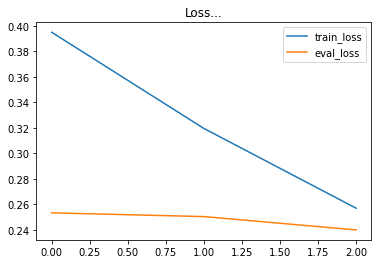
\includegraphics[width=.47\textwidth]{gambar/loss_bert_bahasa.png}
    }
    \subcaptionbox{\textit{Loss} pada model BERT \textit{Multilingual}}{
        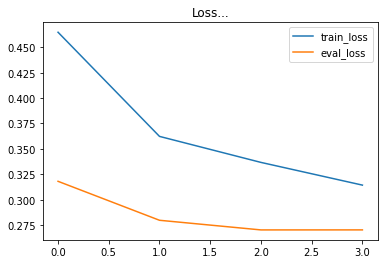
\includegraphics[width=.47\textwidth]{gambar/loss_bert_multilingual.png}
    }
    \subcaptionbox{\textit{Loss} pada model BERT IndoBERT}{
        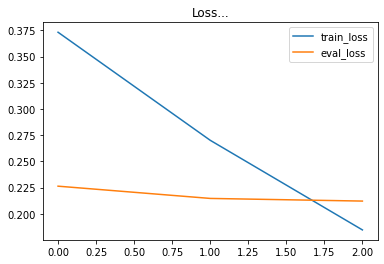
\includegraphics[width=.47\textwidth]{gambar/loss_concat_awal.png}
    }
    \subcaptionbox{\textit{Loss} pada model BERT Cahya 1.5GB}{
        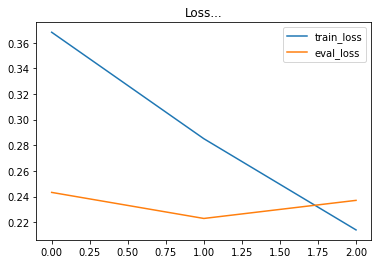
\includegraphics[width=.47\textwidth]{gambar/loss_cahya_bert_1,5.png}
    }
    \subcaptionbox{\textit{Loss} pada model BERT Cahya 522MB}{
        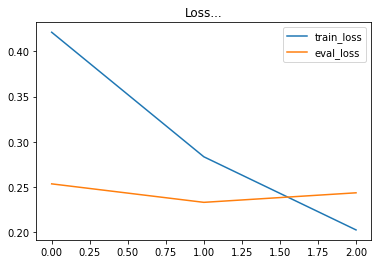
\includegraphics[width=.47\textwidth]{gambar/loss_cahya_bert_522.png}
    }
    \caption{\textit{Loss} pada Model BERT yang digunakan}
    \label{fig:loss_bert_model}
\end{figure}

Dapat dilihat pada gambar \ref{fig:loss_bert_model}, bahwa sebagian besar model BERT memiliki nilai \textit{loss} yang kurang lebih sama. Namun, apabila merujuk pada grafik \textit{loss} yang paling baik dimiliki oleh model \texttt{bert-base-bahasa-standard-case} yang merupakan model yang berisi bahasa Melayu, hal yang sama juga terjadi pada model \texttt{bert-base-multilingual-uncased} yang merupakan model dengan kemampuan \textit{multilanguage}. Sedangkan pada model - model lainnya, sudah mulai terlihat kenaikan pada \textit{validation loss} yang menunjukkan bahwa model sudah mulai mengalami \textit{overfit}.

\begin{figure}[h]
    \centering
    \subcaptionbox{\textit{Confusion Matrix} pada model BERT Bahasa Melayu}{
        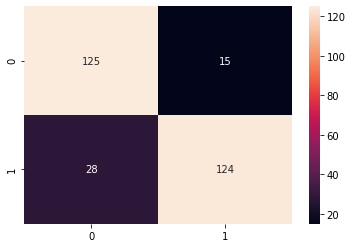
\includegraphics[width=.8\textwidth]{gambar/csf_mat_bert_bahasa.png}
    }
    \subcaptionbox{\textit{Confusion Matrix} pada model BERT \textit{Multilingual}}{
        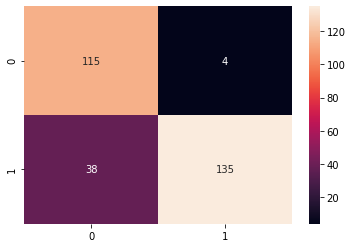
\includegraphics[width=.8\textwidth]{gambar/csf_mat_multilingual.png}
    }
    \caption{\textit{Confusion Matrix} pada Model BERT yang digunakan (bagian 1)}
    \label{fig:cfs_bert_model}
\end{figure}

\begin{figure}[h]
    \centering
    \subcaptionbox{\textit{Confusion Matrix} pada model BERT IndoBERT}{
        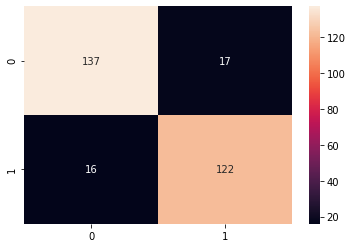
\includegraphics[width=.6\textwidth]{gambar/cfs_mat_concat_awal.png}
    }
    \subcaptionbox{\textit{Confusion Matrix} pada model BERT Cahya 1.5GB}{
        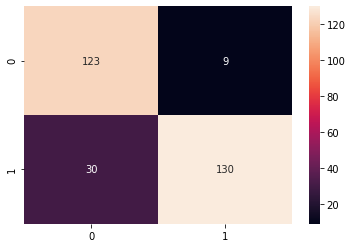
\includegraphics[width=.6\textwidth]{gambar/cfs_matrix_cahya_bert_1,5.png}
    }
    \caption{\textit{Confusion Matrix} pada Model BERT yang digunakan (bagian 2)}
    \label{fig:cfs_bert_model_2}
\end{figure}


\begin{figure}[h]
    \centering
    \subcaptionbox{\textit{Confusion Matrix} pada model BERT Cahya 522M}{
        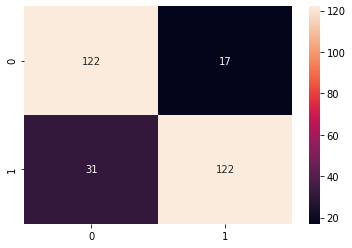
\includegraphics[width=.6\textwidth]{gambar/cfs_matrix_cahya_bert_522.png}
    }
    \caption{\textit{Confusion Matrix} pada Model BERT yang digunakan (bagian 3)}
    \label{fig:cfs_bert_model_3}
\end{figure}
\cleardoublepage

% Bab 5 penutup
\chapter{PENUTUP}
\label{chap:penutup}

% Ubah bagian-bagian berikut dengan isi dari penutup

\section{Kesimpulan}
\label{sec:kesimpulan}

Dari keseluruhan penelitian yang telah dilakukan, maka dapat dimabil beberapa kesimpulan sebagai berikut :

\begin{enumerate}[nolistsep]

  \item Semakin banyak dataset yang digunakan pada waktu \textit{pretrain} BERT, maka semakin akurat juga suatu model tersebut, hal ini terbukti oleh model \textit{indobert-base-p1} yang dilatih dengan 23 GB lebih data.
  \item Metode pemenggalan kata dengan hanya mengambil bagian awal dari suatu teks berhasil memperoleh tingkat akurasi yang lebih baik sebesar 3\% pada hampir seluruh metriks apabila dibandingkan dengan metode - metode pemenggalan teks lainnya. Hal ini karena pada berita berbahasa Indonesia, hampir semuanya diawali dengan \textit{lead} atau inti berita singkat, sehingga dengan mengambil bagian awal saja sudah memadai untuk melakukan klasifikasi.
  \item Penggunaan model BERT yang spesifik untuk bahasa Indonesia secara umum memiliki nilai akurasi yang lebih baik sebesar 10\% pada metriks \textit{precision} apabila dibandingkan dengan model multibahasa maupun bahasa Melayu dalam mendeteksi berita palsu berbahasa Indonesia.
  \item Walaupun sudah terdapat beberapa model lain yang merupakan turunan dari BERT itu sendiri, namun BERT masih merupakan model yang cukup bagus untuk klasifikasi teks, hal ini terlihat dari pengujian dimana BERT memiliki tingkat akurasi yang lebih baik sebesar 1\% dan waktu \textit{training} yang paling sedikit dengan hanya membutuhkan waktu 2 menit 3 detik.
  \item BERT adalah model yang sangat mudah terjadi \textit{overfit}, sehingga pengaturan parameter seperti dengan \textit{dropout} dan parameter \textit{freeze} akan membuat model lebih \textit{general} namun memiliki tingkat akurasi beberapa persen lebih rendah sebesar 5 - 6\% saja.

\end{enumerate}

\section{Saran}
\label{chap:saran}

Adapun dari penelitian ini terdapat beberapa saran dari penulis yang sekiranya dapat membantu untuk meningkatkan hasil dari penelitian ini, saran - saran tersebut adalah :

\begin{enumerate}[nolistsep]

  \item Dataset yang digunakan dalam penelitian ini masih dirasa kurang dan dapat diperbanyak lagi. Semakin banyak dataset yang digunakan semakin bagus pula tingkat akurasi modelnya.
  \item Dataset yang digunakan dalam penelitian ini adalah dataset yang diambil langsung dari situs - situs di internet. Walaupun situs - situs tersebut adalah resmi, namun keabsahan datanya masih harus diverifikasi lagi, lebih spesifik lagi, data dengan label hoaks masih harus diverifikasi lagi.
  \item Salah satu kelemahan BERT adalah jumlah token yang dapat diprosesnya dalam sekali waktu. Sudah terdapat penelitian lain hasil pengembangan dari BERT namun tidak memiliki limitasi jumlah token seperti BERT.
  \item Membuat sistem yang sudah terintegrasi sehingga memudahkan masyarakat dalam mendeteksi berita palsu.

\end{enumerate}

\cleardoublepage

% Daftar pustaka
\renewcommand\bibname{DAFTAR PUSTAKA}
\addcontentsline{toc}{chapter}{\bibname}
\bibliographystyle{unsrtnat}
\bibliography{pustaka/pustaka}
\cleardoublepage

% Biografi penulis
\begin{center}
  \Large
  \textbf{BIOGRAFI PENULIS}
\end{center}

\addcontentsline{toc}{chapter}{BIOGRAFI PENULIS}

\vspace{2ex}

\begin{wrapfigure}{L}{0.3\textwidth}
  \centering
  \vspace{-3ex}
  % Ubah nama file gambar berikut dengan nama file foto dari mahasiswa pertama
  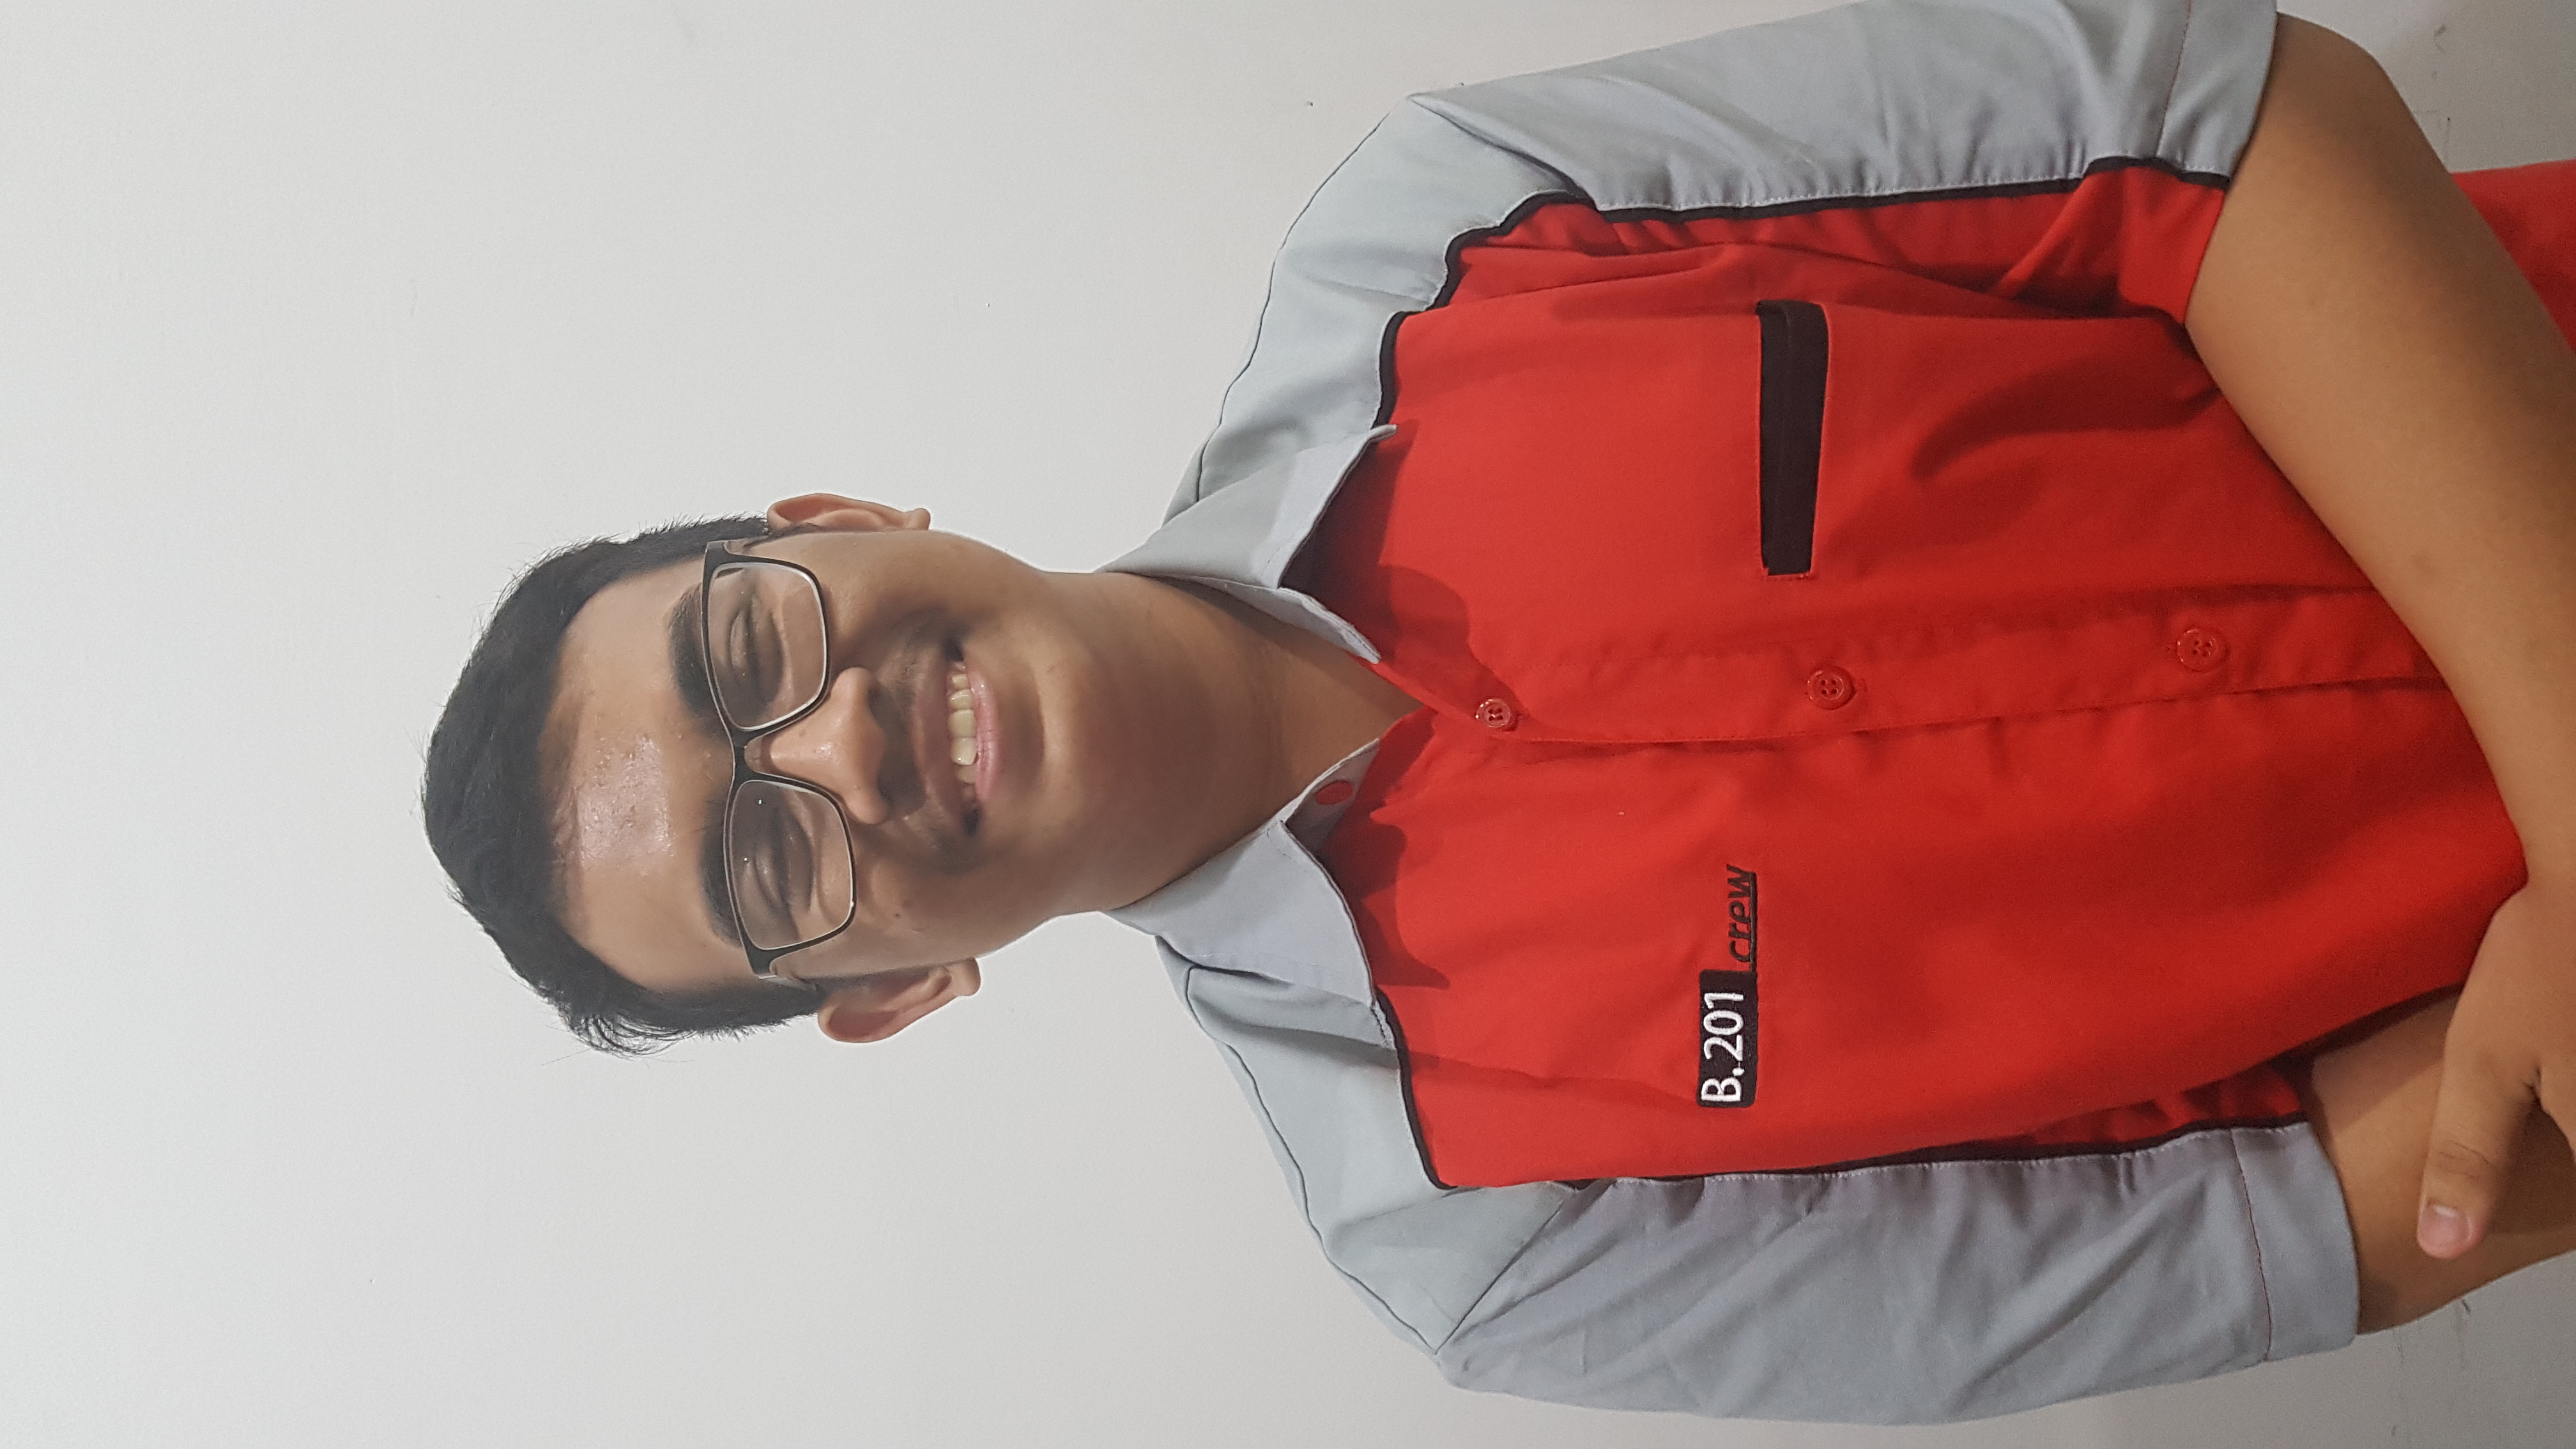
\includegraphics[width=0.5\textwidth, angle=-90]{gambar/foto.jpg}
\end{wrapfigure}

% Ubah kalimat berikut dengan biografi dari mahasiswa pertama
\noindent Aufa Nabil Amiri, lahir pada tanggal 5 Maret 2000, Surabaya. Merupakan seseorang mahasiswa yang berasal dari Institut Teknologi Sepuluh Nopember departemen Teknik Komputer. Penulis merupakan lulusan SMP Muhammadiyah 5 Surabaya dan dilanjutkan dengan SMA Negeri 2 Surabaya. Dalam masa kuliah, penulis tertarik pada bidang pengembangan \textit{Software Development}  dan Pembelajaran Mesin. Selain itu, penulis juga aktif dalam organisasi Lab B201 selama kurang 2 tahun. Penulis juga aktif dalam mengikuti kompetisi pengembangan perangkat lunak dan berhasil meraih penghargaan di ajang GEMASTIK XII 2019. Bagi pembaca yang memiliki kritik, saran, atau pertanyaan mengenai laporan magang ini dapat menghubungi penulis melalui surel aufa.nabil.amiri@gmail.com

\cleardoublepage

\end{document}
